%!LW recipe=pdfLaTeXmk
\documentclass[scheme=plain,aspectratio=169]{beamer}
\usepackage[T1]{fontenc}
\usepackage{fontawesome5}
\usepackage{mathtools}
\usepackage{tikz}
\usepackage{booktabs}
\usepackage{caption}
\usepackage{outlines}
\usepackage{graphicx}
\usepackage{float}
\usepackage{amsthm}
\usepackage{tabularray}
\usepackage{minted}
\usepackage{hyperref}
\usepackage{cleveref}
\usepackage{url}
\usepackage{xspace}
\usepackage{academicons}
\usepackage{pgfplots}
\usepackage{pgfgantt}
\usepackage{qrcode}
\usepackage{ninecolors}
\usepackage{soul}
\usepackage{tgheros}
\usepackage{xparse}
\usepackage[
  citestyle=authoryear,
  bibstyle=authoryear,
  backend=biber,
  url=false,doi=false,isbn=false
]{biblatex}
\newmintinline[code]{html}{fontsize=\small}
\addbibresource{yuxuan.bib}
\addbibresource{custom.bib}
\DeclareCiteCommand{\silentfootcitetext}
  {\usebibmacro{prenote}}
  {\printtext[bibhyperref]{%
     \printnames{labelname}%
     \addcomma\space
     \usebibmacro{cite:labeldate+extradate}%
     \iffieldundef{booktitle}
       {\iffieldundef{journaltitle}
          {\iffieldundef{eprint}
             {}
             {\addcomma\space
              \iffieldundef{archiveprefix}
                {\printfield{eprint}}
                {\printfield{archiveprefix}\addcolon\printfield{eprint}}}}
          {\addcomma\space\printfield{journaltitle}}}
       {\addcomma\space\printfield{booktitle}}}}
  {\multicitedelim}
  {\usebibmacro{postnote}}
\newcommand{\silentfootcite}[1]{%
  {%
    \setbeamertemplate{footnote}{%
      \parindent 0em\noindent\raggedright\insertfootnotetext\par%
    }%
    \footnotetext{\silentfootcitetext{#1}}%
  }%
}
\newcommand{\todo}[1]{\sethlcolor{red!30!white}\hl{#1}}

\usetheme[
    progressbar=frametitle,
    numbering=fraction,
    subsectionpage=progressbar,
    titleformat title=smallcaps,
    titleformat subtitle=smallcaps,
    titleformat section=smallcaps,
    titleformat frame=smallcaps]{moloch}

\setbeamercolor{palette primary}{bg=gray1}
\setbeamercolor{frametitle}{bg=black,fg=white}
\setbeamercolor{progress bar}{fg=black}
\setbeamerfont{footnote}{size=\tiny}
\renewcommand{\cite}{\footcite}

\definecolor{ForestGreen}{RGB}{34,139,34}
\newcommand{\highlightRelevantValue}[1]{%
  \ifdim #1pt > 0pt
    {\color{ForestGreen}{#1\%}}%
  \else
    {\color{red}{#1\%}}%
  \fi
}


\NewDocumentCommand{\imageframe}{m O{1}}{
  \begin{frame}[plain]
    \begin{tikzpicture}[remember picture,overlay]
      \node[anchor=center, inner sep=0] at (current page.center) {
        \includegraphics[
          width=#2\paperwidth,
          height=#2\paperheight,
          keepaspectratio
        ]{#1}
      };
    \end{tikzpicture}
  \end{frame}
}

\usetikzlibrary{calc}
\setcounter{tocdepth}{1}

\makeatletter
\newlength{\frametitle@padding}
\setlength{\frametitle@padding}{2.2ex}
\newcommand{\frametitlestrut@start}{
  \rule{0pt}{\frametitle@padding +%
    \totalheightof{%
      \ifcsdef{frametitleformat}{\frametitleformat X}{X}%
    }%
  }%
}

\newcommand{\frametitlestrut@end}{
  \rule[-\frametitle@padding]{0pt}{\frametitle@padding}
}

\setbeamertemplate{frametitle}{
    \nointerlineskip%
    \begin{beamercolorbox}[%
        wd=\paperwidth,%
        sep=0pt,%
        leftskip=\frametitle@padding,%
        rightskip=\frametitle@padding,%
      ]{frametitle}%
    \frametitlestrut@start%
    \insertframetitle%
    \hfill%
    \nolinebreak%
    \frametitlestrut@end%
    \end{beamercolorbox}%
    \begin{tikzpicture}[remember picture,overlay]
        \coordinate (logo) at ([xshift=-1.8cm,yshift=-0.5cm]current page.north east);
        \node at (logo) {
\includegraphics[height=.1\textheight]{figures/webserv/northeastern.eps}};
    \end{tikzpicture}
}
\makeatother


\setbeamertemplate{footline}{
    \hbox{
    \begin{beamercolorbox}[wd=\paperwidth,ht=3ex,dp=1.5ex,leftskip=2ex,rightskip=2ex]{page footer}%
        \usebeamerfont{title in head/foot}%
        \hfill
        \begin{tblr}{
            width=.8\linewidth,
            colspec={X[5,l]X[r]}
        }
            \insertsectionhead{}
            % &
            % \ifx\insertsubsection\empty
            % \else
            % \insertsubsection{} 
            % \fi
            &
            \insertframenumber{} / \inserttotalframenumber
        \end{tblr}
        \hfill{}
    \end{beamercolorbox}}%
}


\defbeamertemplate{section page}{my progressbar}{
  \centering
  \begin{beamercolorbox}[wd=\paperwidth,leftskip=10mm,rightskip=10mm,sep=0pt]{section page}
    \begin{minipage}{0.9\linewidth}
      \raggedright
      \usebeamercolor[fg]{section title}
      \usebeamerfont{section title}
      \insertsection\\[-0.5\baselineskip]
      \usebeamertemplate*{progress bar in section page}
      \par
      \usebeamercolor[fg]{subsection title}%
      \usebeamerfont{subsection title}%
      \strut\ifx\insertsubsectionhead\@empty\else\insertsubsectionhead\fi
    \end{minipage}
  \end{beamercolorbox}
  \par
}
\setbeamertemplate{section page}[my progressbar]

\UseTblrLibrary{booktabs}
\graphicspath{ {./figures/} {./figures/uxagent/} {./figures/finetuned_web_agent/} {./figures/webserv/} }

\DeclareRobustCommand{\projectname}{\textsc{WebServ}\xspace}

\title{Human–AI Collaboration for UX Research}
\subtitle{Designing, Evaluating, and Improving LLM Agents as Simulated Users}

\author{\textbf{Yuxuan Lu}}
\institute{Northeastern University \quad | \quad \url{https://yuxuan.lu} \quad | \quad lu.yuxuan@northeastern.edu}
\date{Mar 2026}
\begin{document}


\maketitle

\section*{Introduction}


\begin{frame}{About Me}
  \textbf{Yuxuan (Leo) Lu} \hfill \url{https://yuxuan.lu} \\
  Ph.D. student, Northeastern University (Khoury) --- advised by Prof. Dakuo Wang \\

  \textbf{Industry Experience:} Applied Scientist Intern at Amazon (Sep 2024--present); ML Research Intern at LinkedIn China (Jul 2022--May 2023).


  \textbf{Research Focus:} I work at the intersection of NLP and HCI.


\end{frame}

\begin{frame}{Selected Works}

  % \vspace{10pt}
  \begin{columns}[t]
    \begin{column}{0.48\linewidth}
      \begin{tblr}{colspec={lr},row{1}={font=\bfseries}}
        NLP Works \\
        SFT LLM Agent & ACL'26 \\
        WebServ & preprint \\
        \\
      \end{tblr}
    \end{column}

    \begin{column}{0.48\linewidth}
      \begin{tblr}{colspec={lr},row{1}={font=\bfseries}}
        HCI Works \\
        UXAgent & CHI'25 LBW \\
        Agent A/B & CHI'26 Posters \\
        UXAgent & UIST'26 under review \\
      \end{tblr}
    \end{column}
  \end{columns}

  \vspace{4pt}
  Co-authored: 6 accepted NLP papers (ICLR/EMNLP/NAACL/ACL), 4 accepted HCI papers (CHI/CSCW/UbiComp), plus 3 NLP and 1 HCI papers under review.
\end{frame}


{
\setbeamercolor{background canvas}{bg=white}
\begin{frame}[plain]
  \begin{figure}[htp]
    \centering
    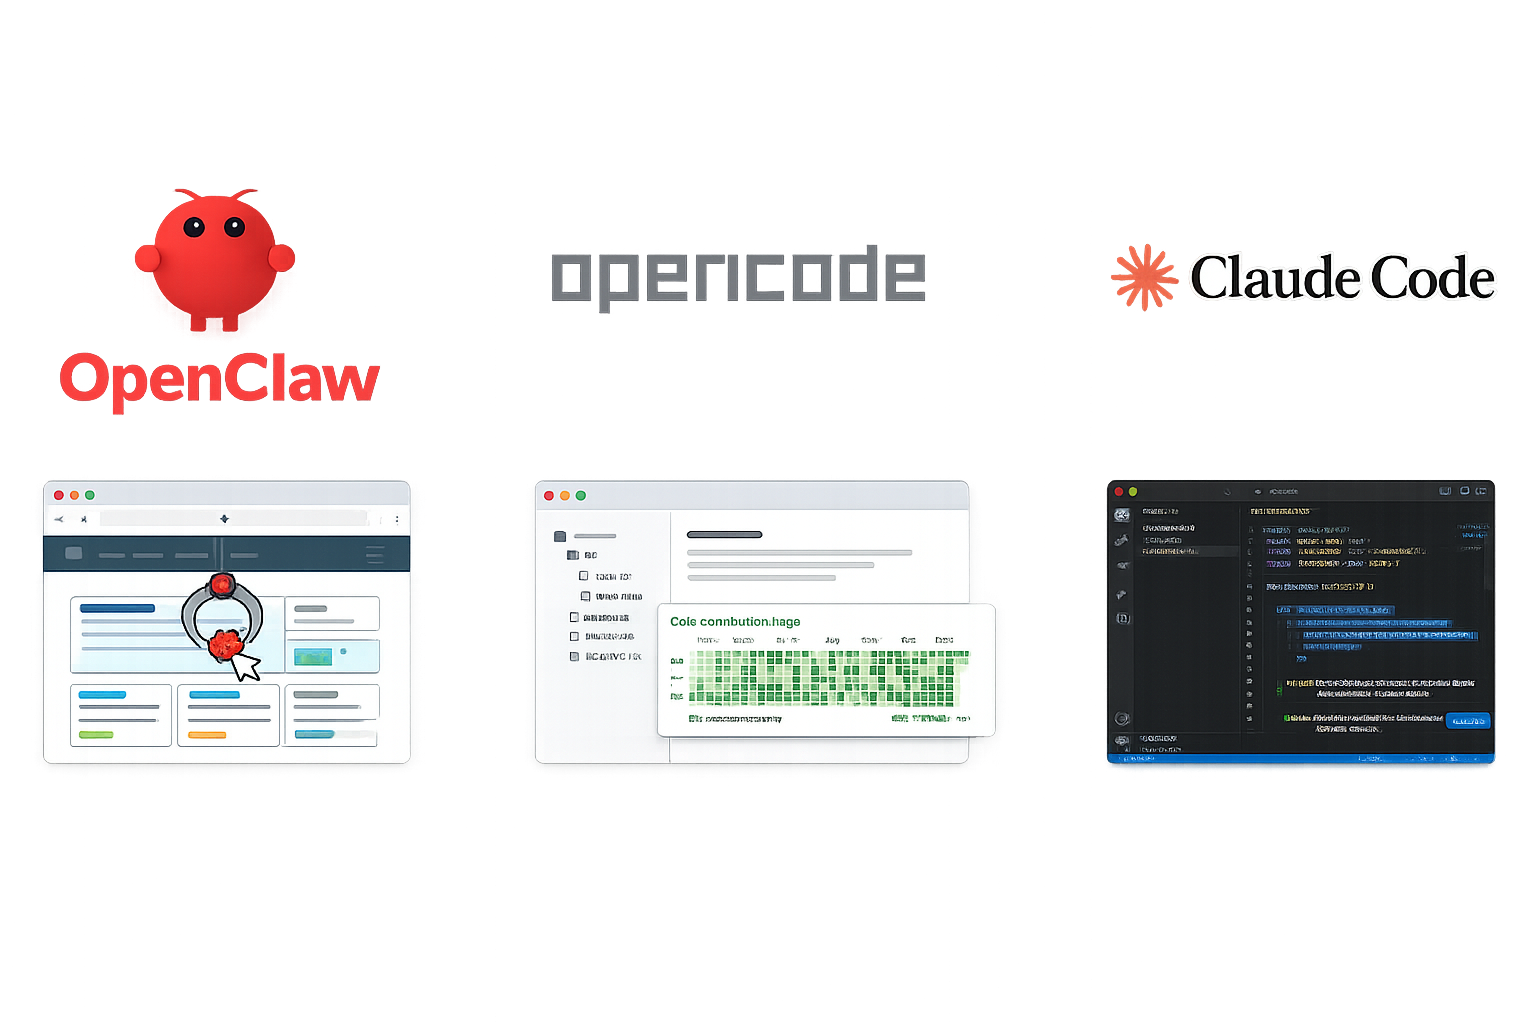
\includegraphics[width=.8\linewidth]{agents.png}
  \end{figure}
\end{frame}

\begin{frame}[plain]
\begin{figure}[htp]
  \centering
  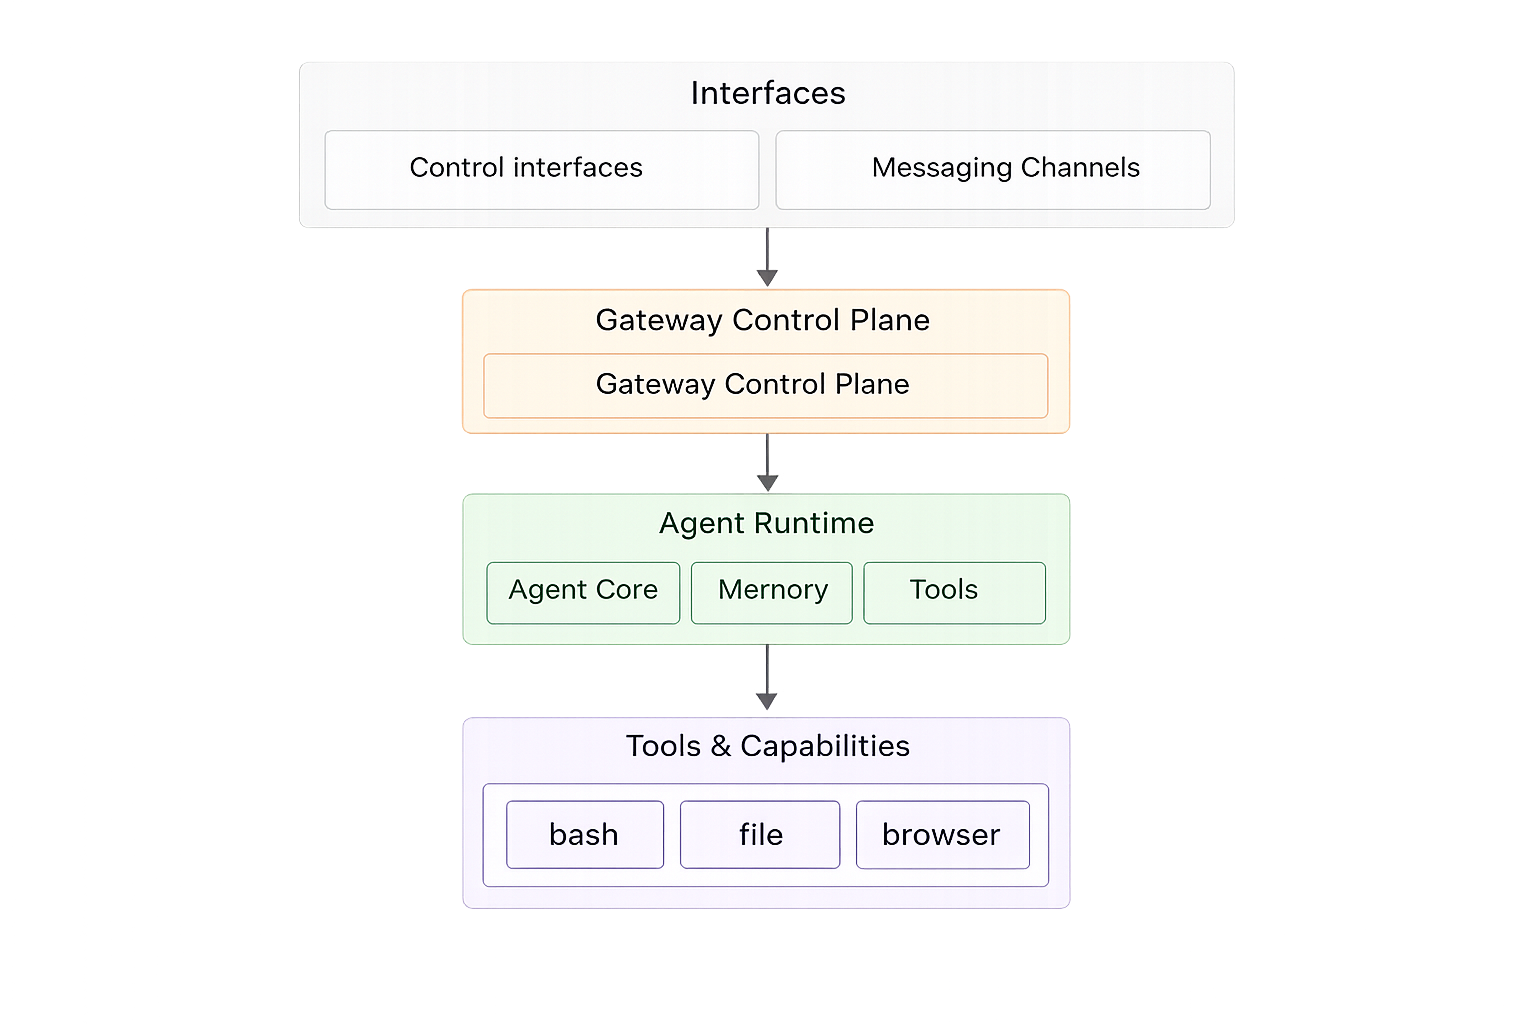
\includegraphics[width=.8\linewidth]{openclaw.png}
\end{figure}
\end{frame}

{
\definecolor{bgdark}{HTML}{121212}
\setbeamercolor{background canvas}{bg=bgdark}
\begin{frame}[plain]
  \begin{tikzpicture}[remember picture,overlay]
    \node[anchor=center, inner sep=0] at (current page.center) {
      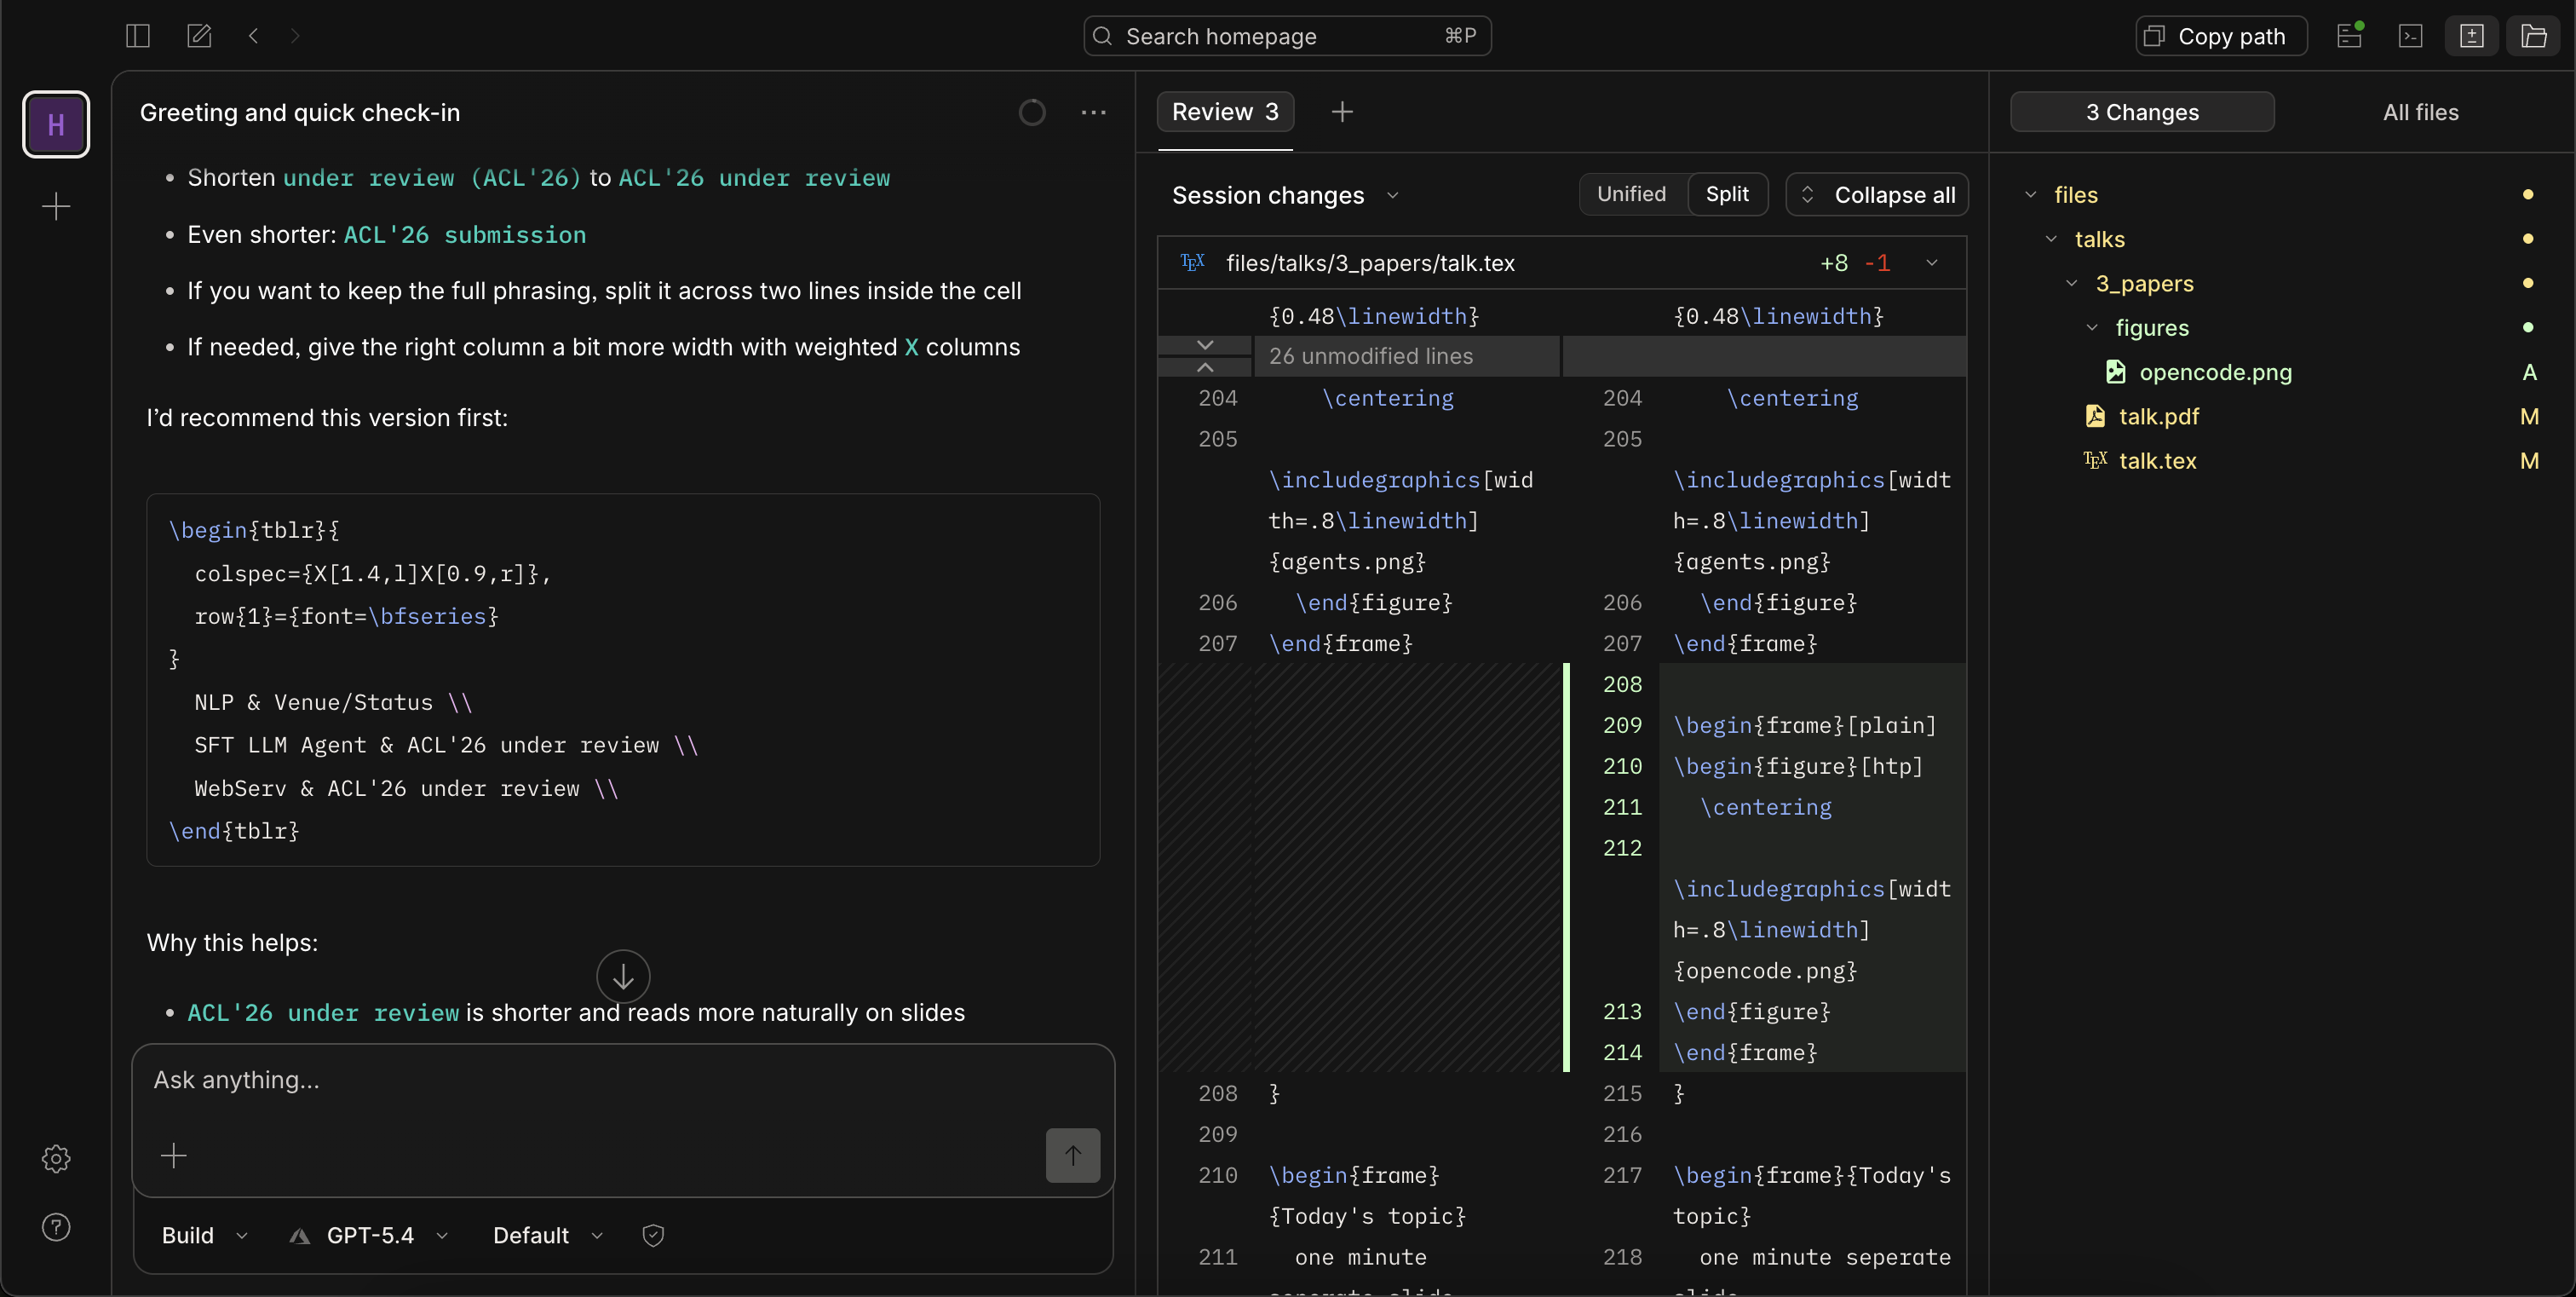
\includegraphics[
        width=\paperwidth,
        height=\paperheight,
        keepaspectratio
      ]{opencode-screenshot.png}
    };
  \end{tikzpicture}
\end{frame}
}

{%


\begin{frame}{What’s the worst nightmare for a researcher?}
  \begin{outline}
    \1 Spending weeks on a study, only to find that the results are not significant
    \1 Training a model for days, only to find a bug in your preprocessing pipeline
    \1 Realizing that your experiment design is flawed one week before deadline
  \end{outline}
\end{frame}

\begin{frame}{As someone from both NLP and HCI, I think …}
\begin{table}
  \centering
  \begin{booktabs}{
    colspec = {ccc},
    width = \linewidth,
    cells={m},
  }
  \toprule
   & NLP & HCI \\
  \midrule
  Experiment Subject & Models and Machines & Human Subjects \\
  Experiment Design &  Code and Data & Study Protocol \\
  Experiment Cost & Money & Human Participants' Time \\
  ``Debugging'' Method & Code Debugging & ??? \\
  \bottomrule
  \end{booktabs}
\end{table}
\pause
\begin{center}
  \Large
  \textbf{Human Participants' Time is Valuable and Limited}
\end{center}
\end{frame}

\setbeamercolor{background canvas}{bg=white}
\begin{frame}[plain]
  \begin{figure}[htp]
    \centering
    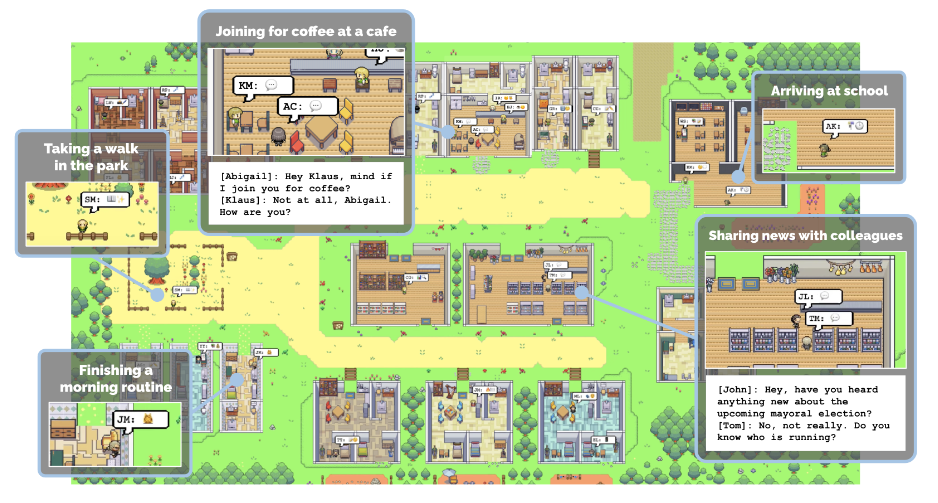
\includegraphics[width=\linewidth]{figures/uxagent/stanford.png}
  \end{figure}
  \silentfootcite{parkGenerativeAgentsInteractive2023}
\end{frame}

\begin{frame}[plain]
  \begin{figure}[htp]
    \centering
    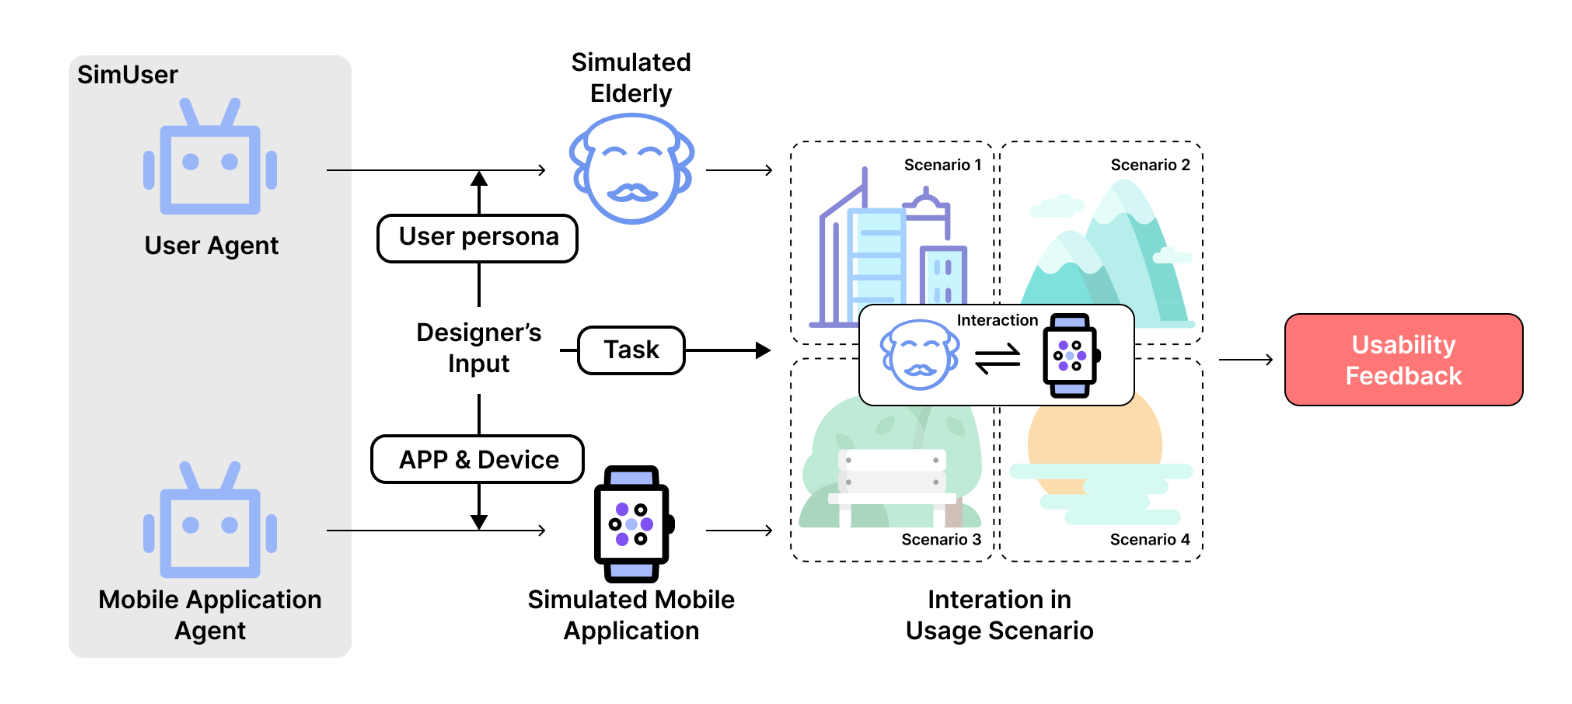
\includegraphics[width=\linewidth]{simuser.png}
  \end{figure}
  \silentfootcite{xiangSimUserGeneratingUsability2024}
\end{frame}

\begin{frame}[plain]
  \begin{figure}[htp]
    \centering
    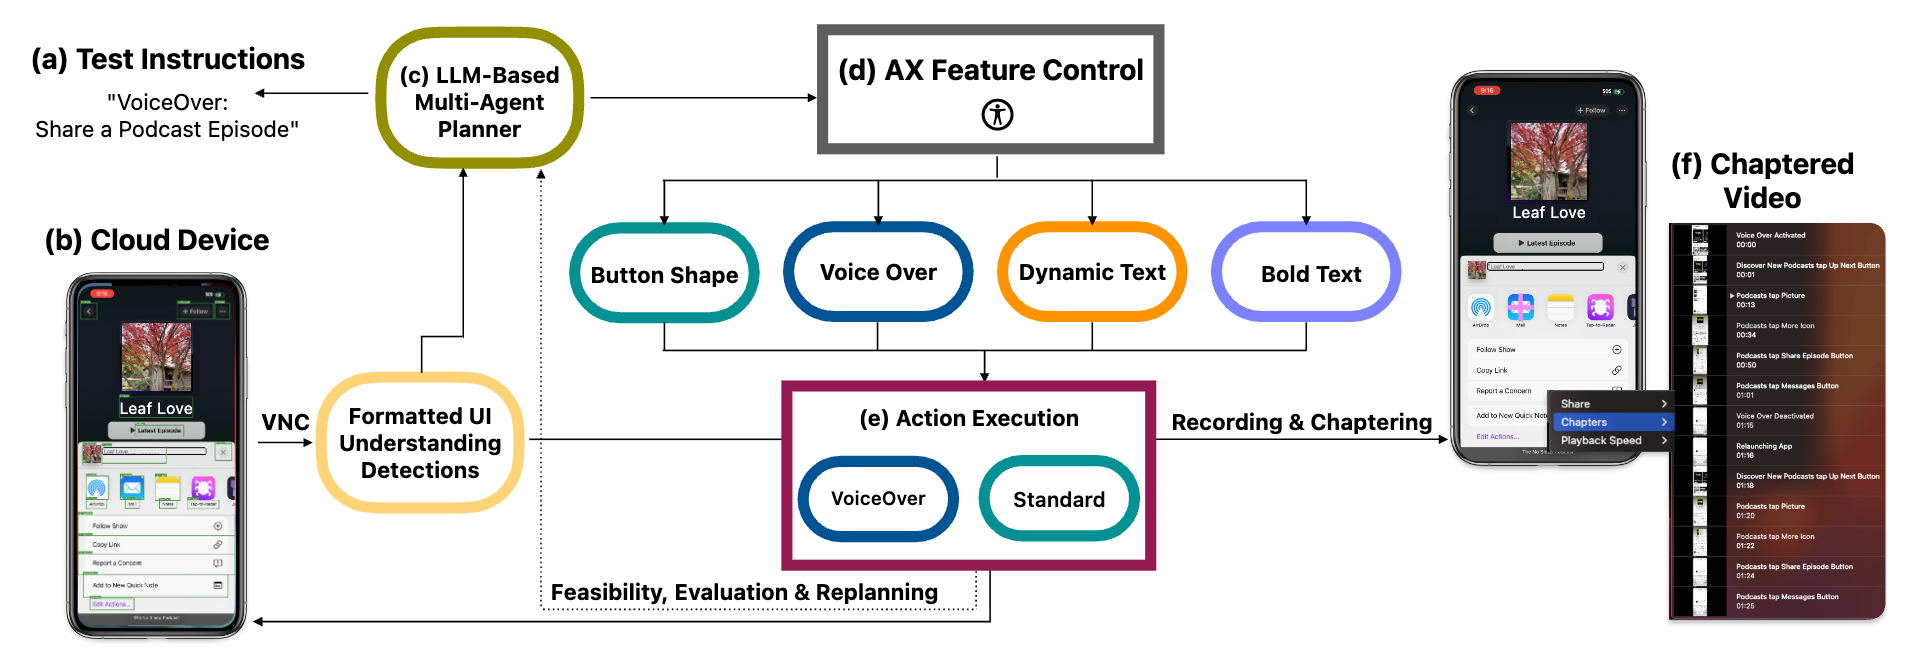
\includegraphics[width=\linewidth]{axnav.png}
  \end{figure}
  \silentfootcite{taebAXNavReplayingAccessibility2024}
\end{frame}


\begin{frame}[plain]
  \begin{figure}[htp]
    \centering
    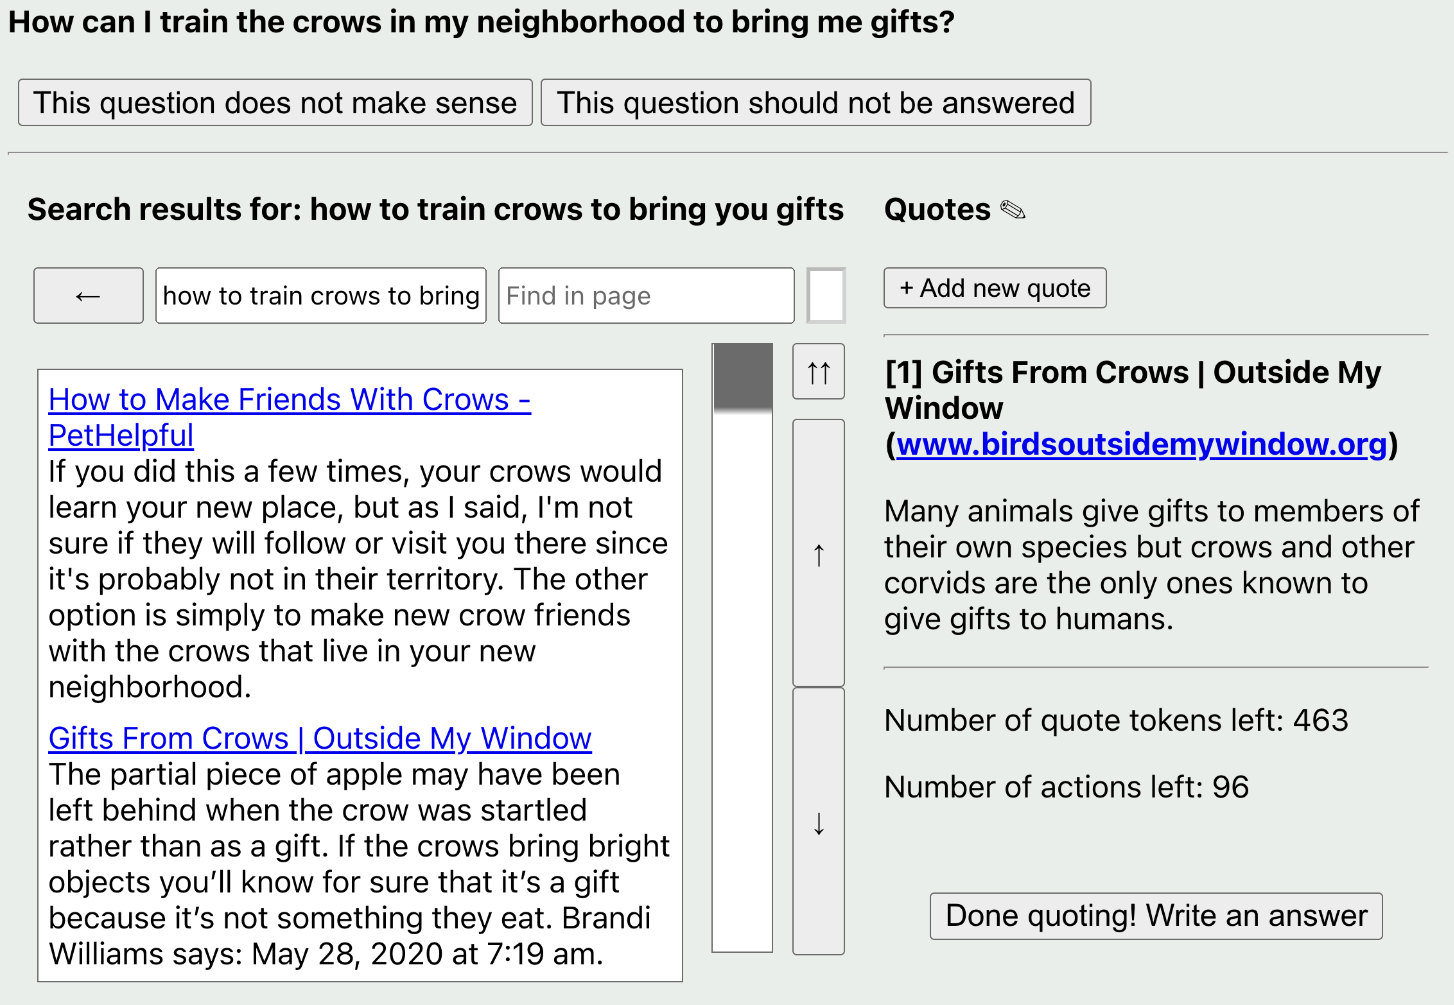
\includegraphics[width=.8\linewidth]{webgpt.png}
  \end{figure}
  \silentfootcite{nakanoWebGPTBrowserassistedQuestionanswering2022}
  \end{frame}
  
  \begin{frame}[plain,c]
    \begin{figure}[htp]
      \centering
      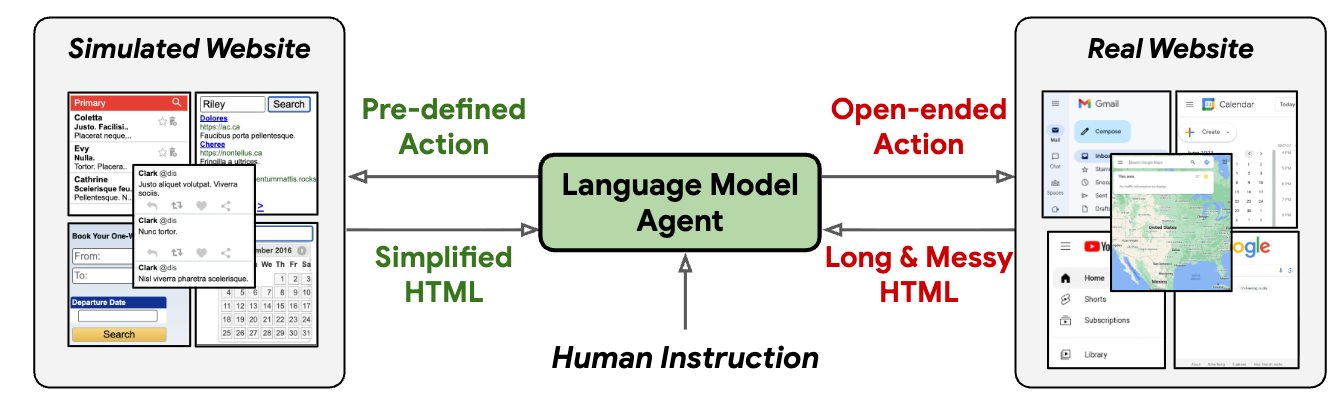
\includegraphics[width=.8\linewidth]{webagent.png}
      \caption{WebAgent, ICLR 2024}
    \end{figure}  
    \silentfootcite{gurRealWorldWebAgentPlanning2023}
  \end{frame}
}


\begin{frame}{Challenges}
  \begin{figure}[htp]
    \centering
    
\includegraphics[width=.5\linewidth]{challenge-sandbox.png}
  \end{figure}
  Existing LLM Agent systems mostly works in \textbf{sandboxed environments}
\end{frame}

\begin{frame}{Challenges}
  \begin{columns}[c]
    \begin{column}{0.48\linewidth}
\begin{figure}[htp]
  \centering
  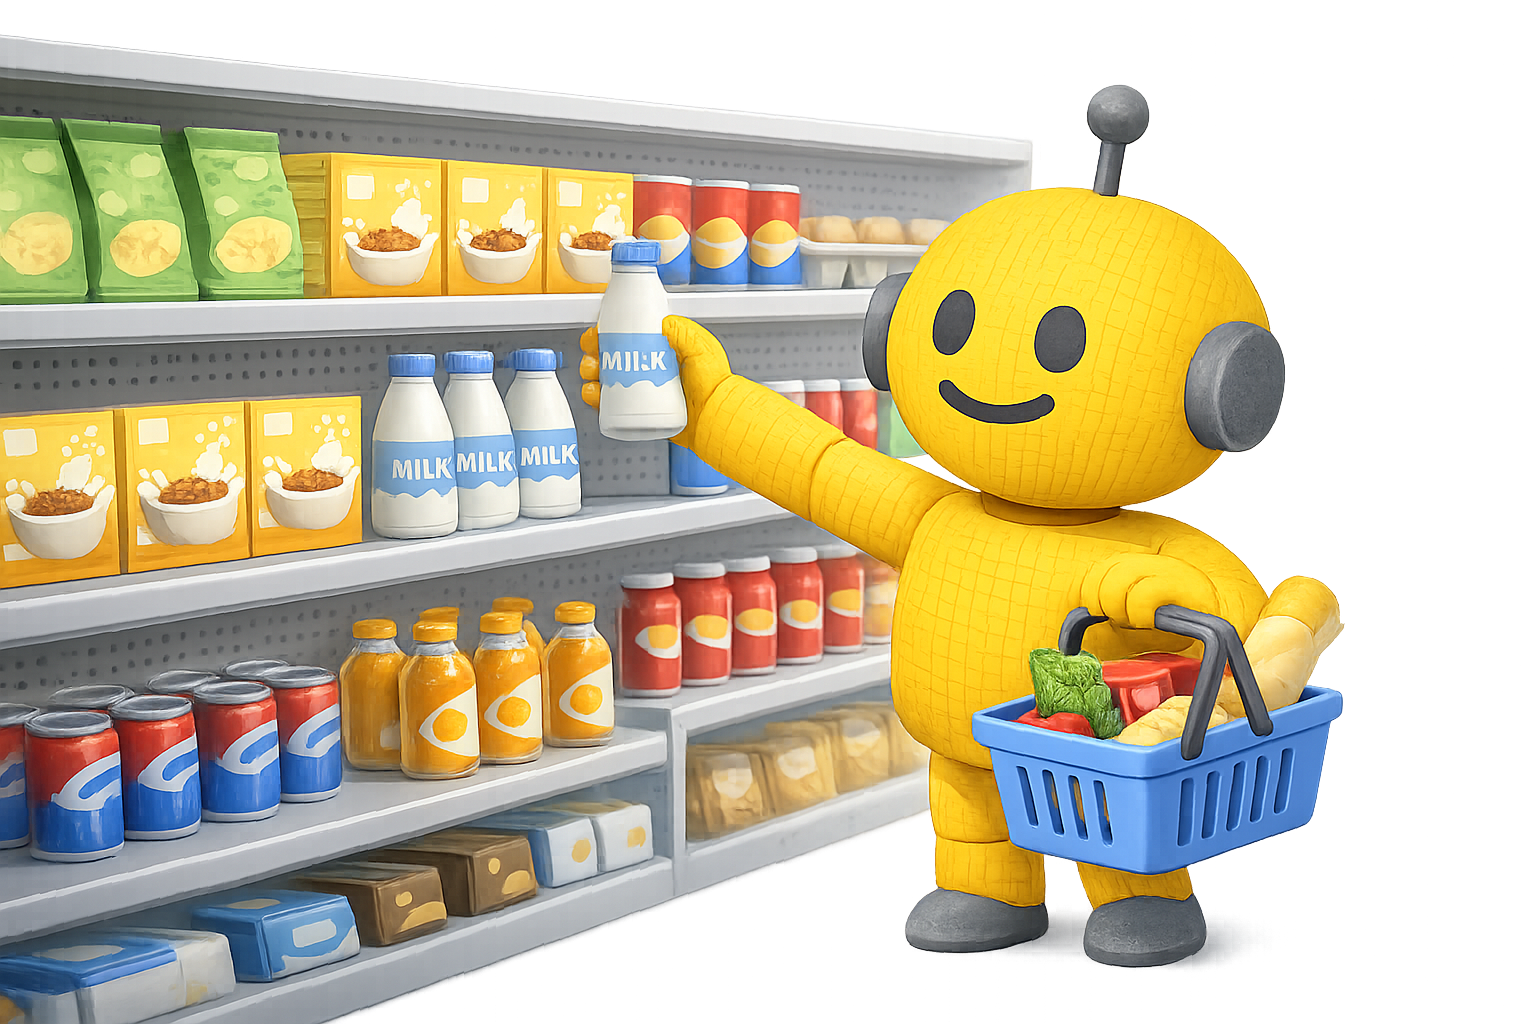
\includegraphics[width=\linewidth]{challenge-agent.png}
\end{figure}
    \end{column}
    \begin{column}{0.48\linewidth}
     \begin{figure}[htp]
        \centering
        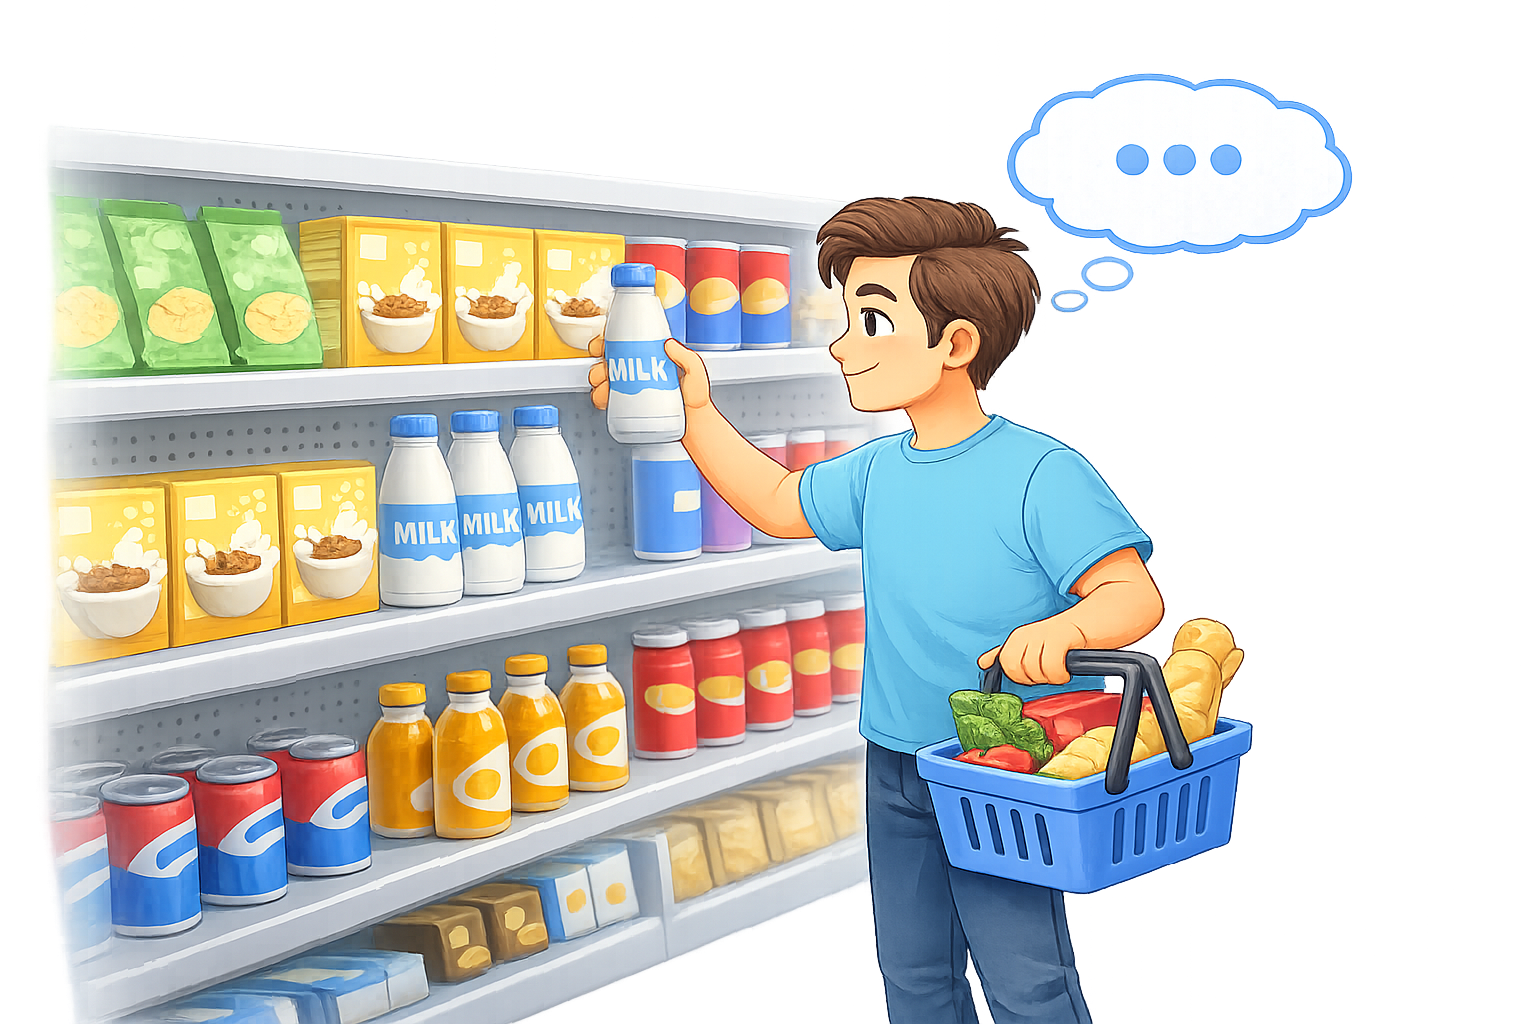
\includegraphics[width=.8\linewidth]{challenge-user.png}
      \end{figure}
    \end{column}
  \end{columns}
\end{frame}


\begin{frame}[standout]
  How can we \ul{design} LLM agent systems for UX research?
  \begin{figure}[htp]
    \centering
    
\includegraphics[width=.4\linewidth]{puzzled-agent.png}
  \end{figure}
\end{frame}




\begin{frame}[standout]
  How can we \ul{evaluate} LLM agent systems?
  \begin{figure}[htp]
  \centering
  
\includegraphics[width=.4\linewidth]{evaluate-agent.png}
  % \caption{}
\end{figure}
\end{frame}



\begin{frame}[standout]
  How can we \ul{improve} LLM agent systems?
\begin{figure}[htp]
  \centering
  
\includegraphics[width=.4\linewidth]{improve-agent.png}
  % \caption{}
\end{figure}
\end{frame}
}

% \begin{frame}{Today's topic}
%   one minute seperate slide 

%   Motivation for three work; one page introduction overall motivation for 3 works. Maybe start from openclaw -- what it can do . our work started ... same as openclaw .. if you think about openclaw, you nede to design: 
%   agent system
%   browser connector
%   training environment

%   we don't know how well ...

%   how can we improve model. 

%   don't equally distribute time for 3 case studies. 

%   5-8 for intro and motivation; 10 minute for one ; 3  - 5 for other two.

%   \begin{enumerate}

%     \item \textbf{Designing} LLM agent system for UX research 
%     \item \textbf{Evaluating} how well llm agent model simulate real users
%     \item \textbf{Improving} them with Reinforcement Learning infra
%   \end{enumerate}
% \end{frame}

\section[Case Study 1: UXAgent]{Case Study 1: UXAgent: A System for Simulating Usability Testing of Web Design with LLM Agents}

% \begin{frame}{What’s the worst nightmare for a researcher?}
%   change to UX Researcher, change to undergrad friendly version
%   \begin{outline}
%     \1 The myth of “Reviewer 2”
%     \1 Paper being scooped
%     \1 Realizing that your experiment design is flawed one week before deadline
%   \end{outline}
% \end{frame}


\begin{frame}[standout]
  How can we better evaluate UX Research study design before running the study?
\end{frame}

\begin{frame}[standout]
  How can we better evaluate \ul{usability} testing study design before running the study
\end{frame}

% \begin{frame}{Challenges}
%   change to figure
%   \begin{outline} 
%     \1 Existing LLM Agent systems mostly works in \textbf{sandboxed environments}
%     \1 Existing LLM Web Agents focus on \textbf{task completion rate}, not simulating complex and dynamic human behavior
%     \1 Existing reasoning architecture of LLM Agents/LLM Web Agents either fail to simulate human reasoning process (too simple) or introduces additional latency (too complex) for real time simulation. 
%   \end{outline}
% \end{frame}

\begin{frame}{Our Solution: UXAgent}
\begin{figure}[htp]
  \centering
    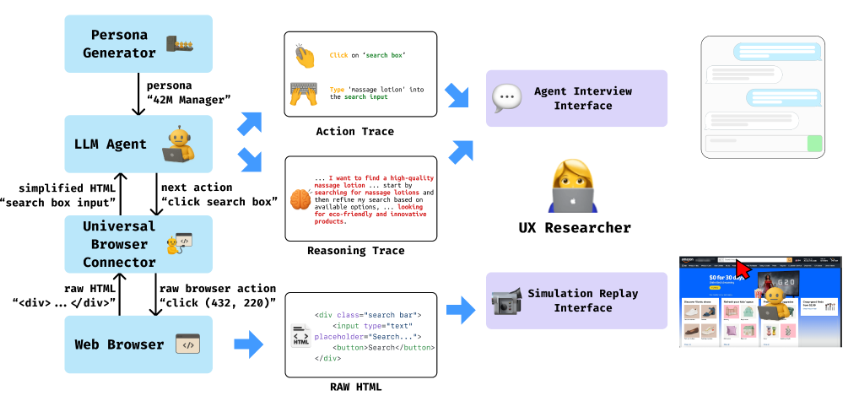
\includegraphics[width=.8\linewidth]{figures/uxagent/uxagent.png}
  \caption{System Architecture of UXAgent}
\end{figure}
\url{https://www.youtube.com/watch?v=-2xpeJ04mRA}
\end{frame}

% \begin{frame}[standout]

%   \begin{figure}[htp]
%     \centering
%     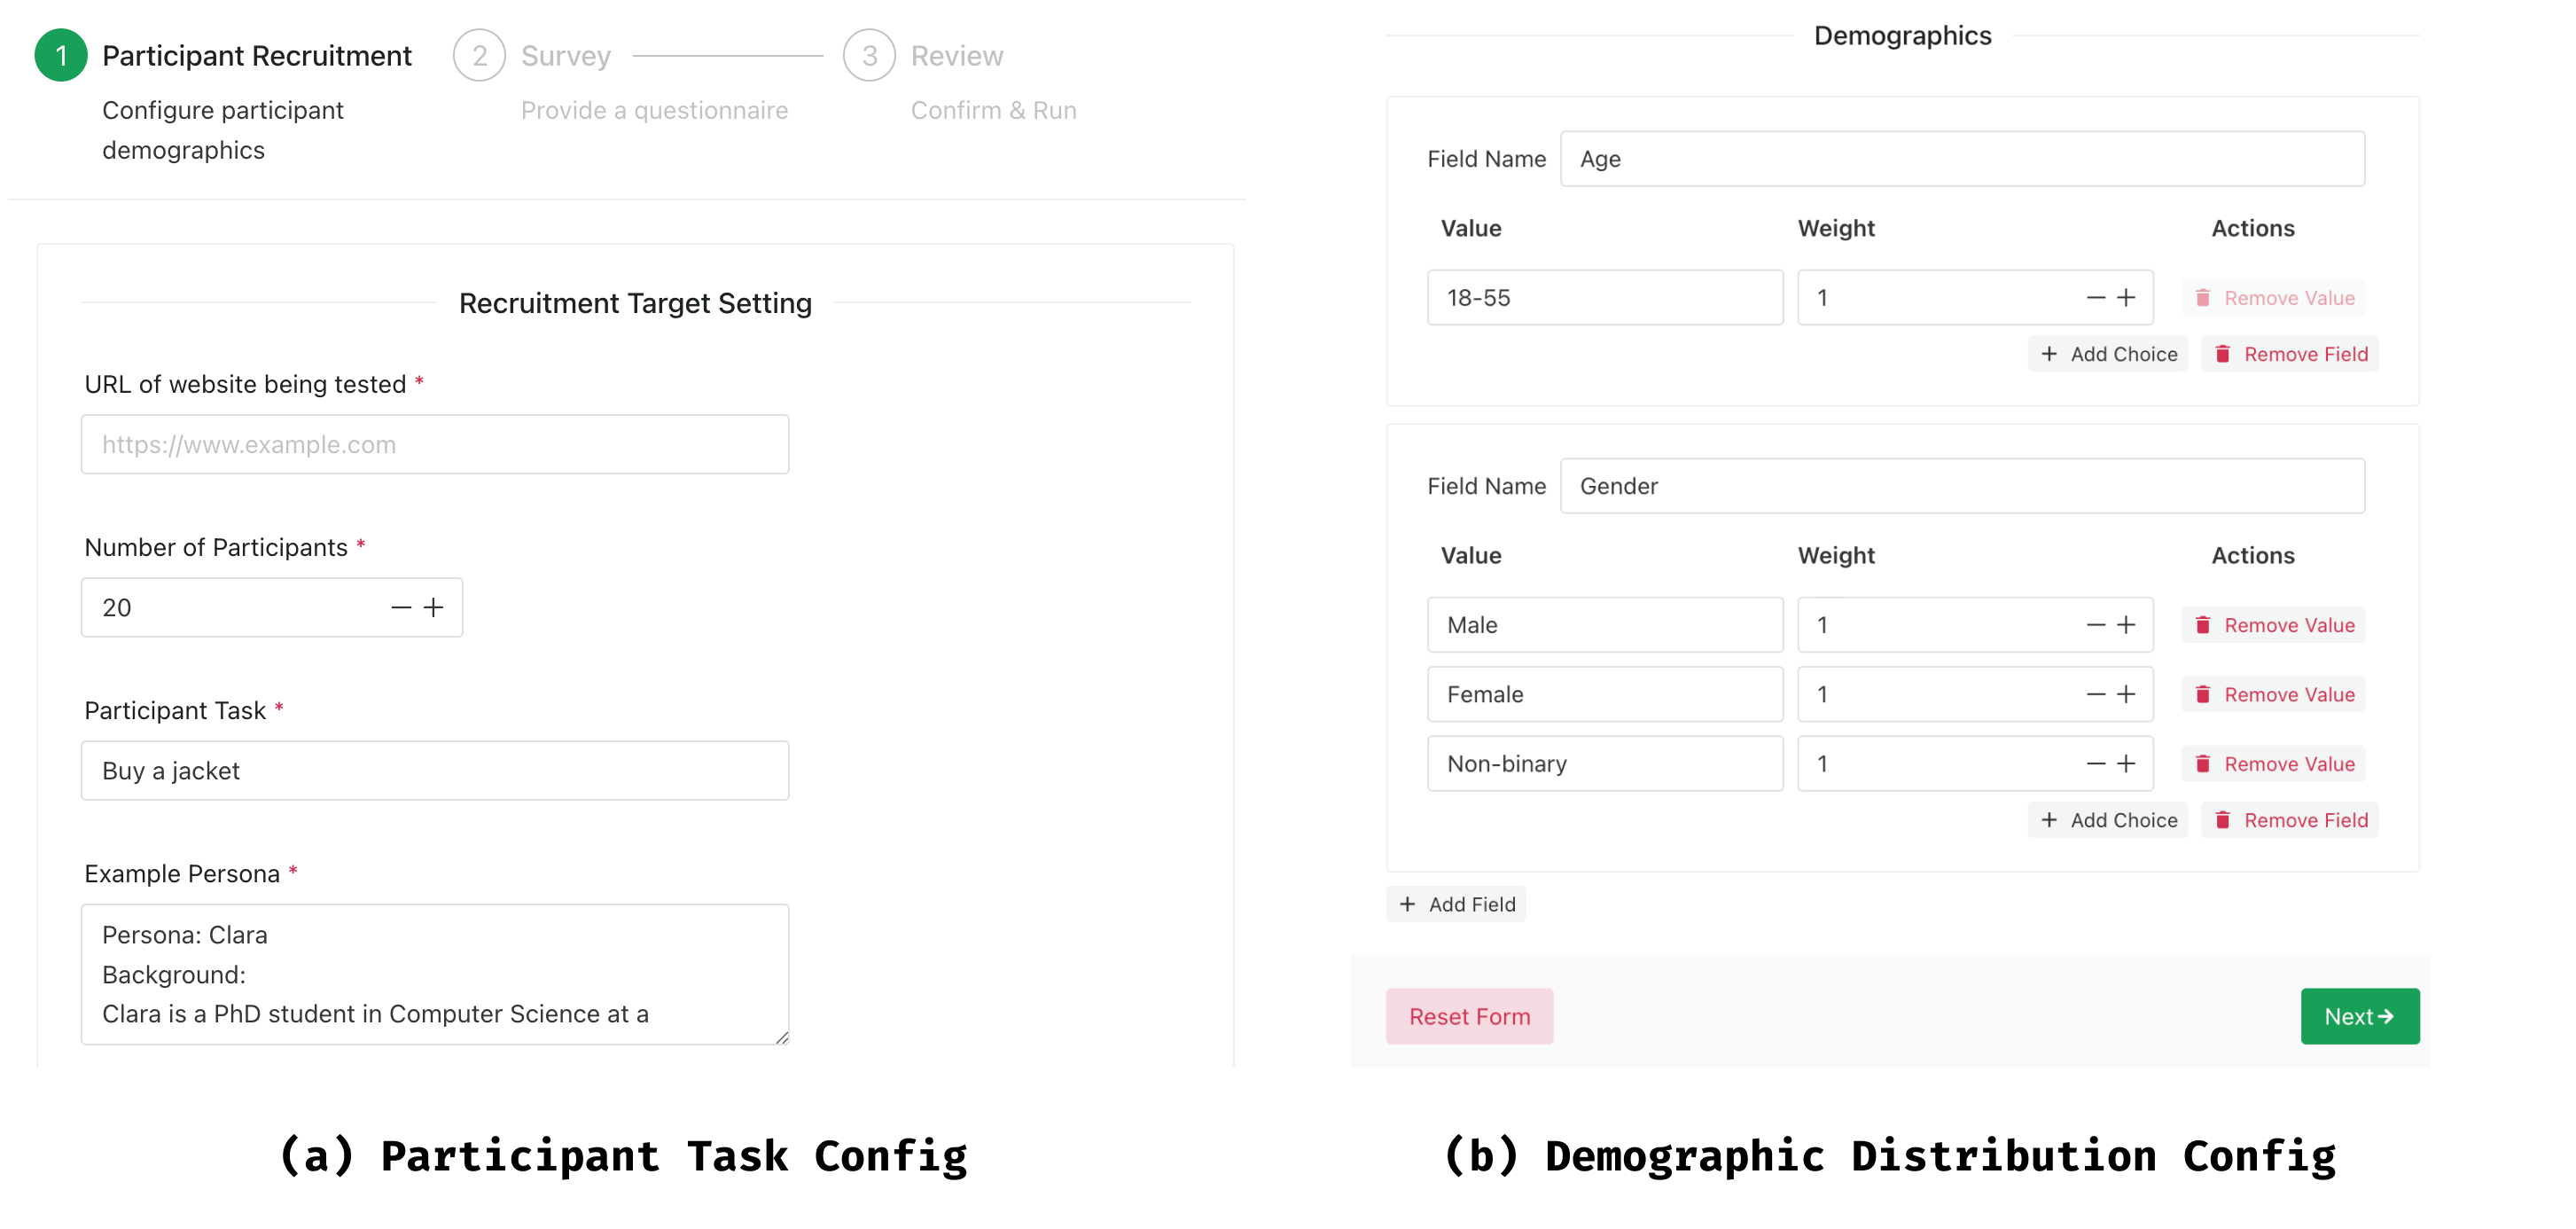
\includegraphics[width=\paperwidth]{figures/uxagent/study_configure_interface.png}
%   \end{figure}
% \end{frame}
\imageframe{figures/uxagent/study_configure_interface.png}[1]

% Agent Archite
\begin{frame}{Agent Architecture}
  \begin{figure}[htp]
    \centering
    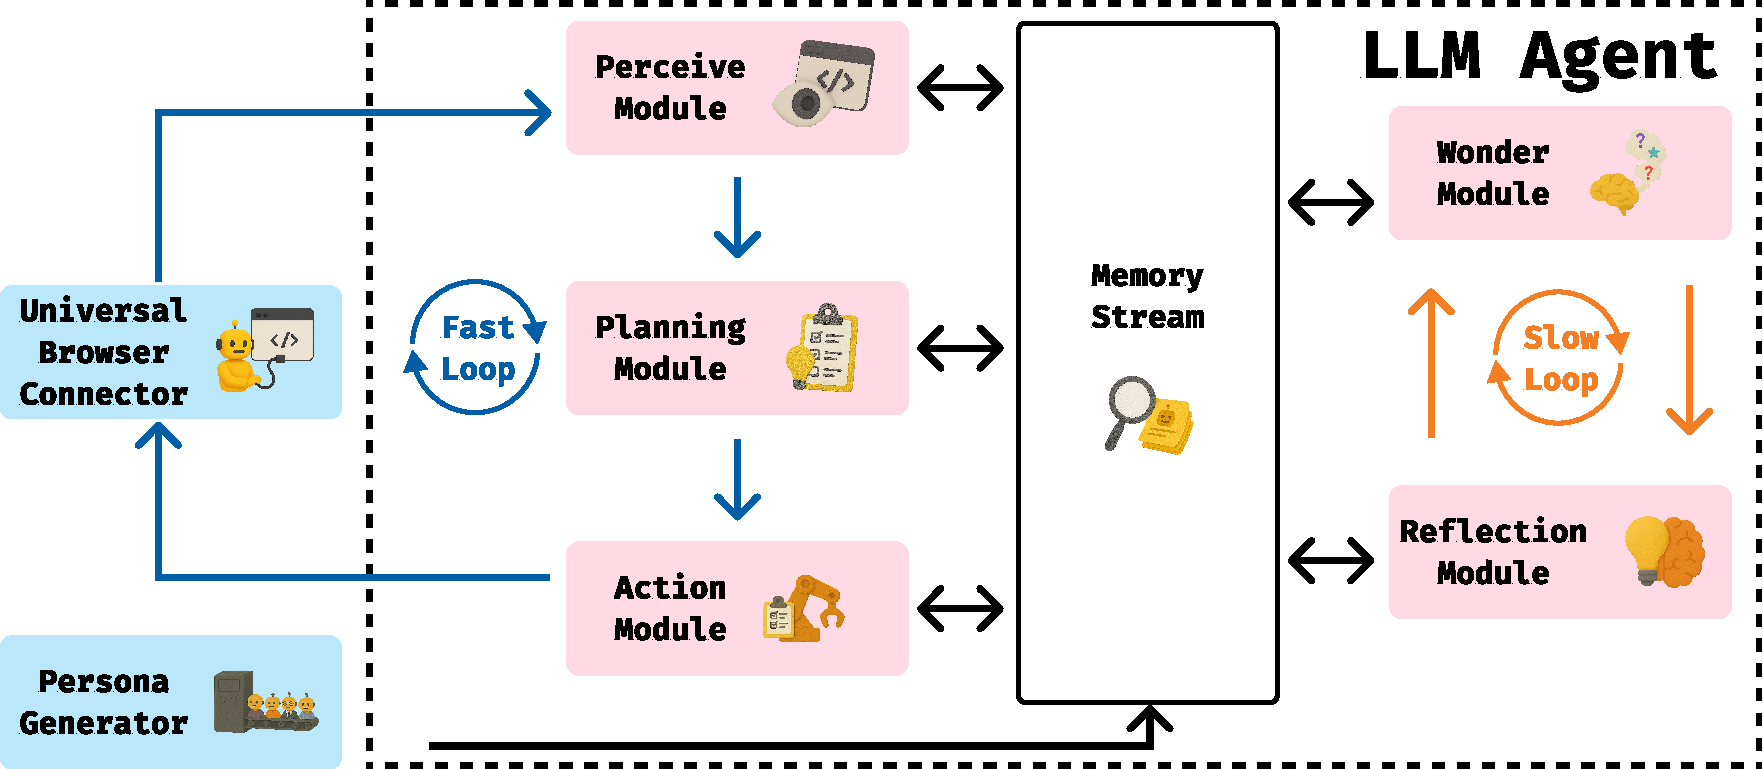
\includegraphics[width=\linewidth]{figures/uxagent/structure.pdf}
  \end{figure}
\end{frame}
\begin{frame}{Agent Architecture - Fast Loop}
  \begin{figure}[htp]
    \centering
    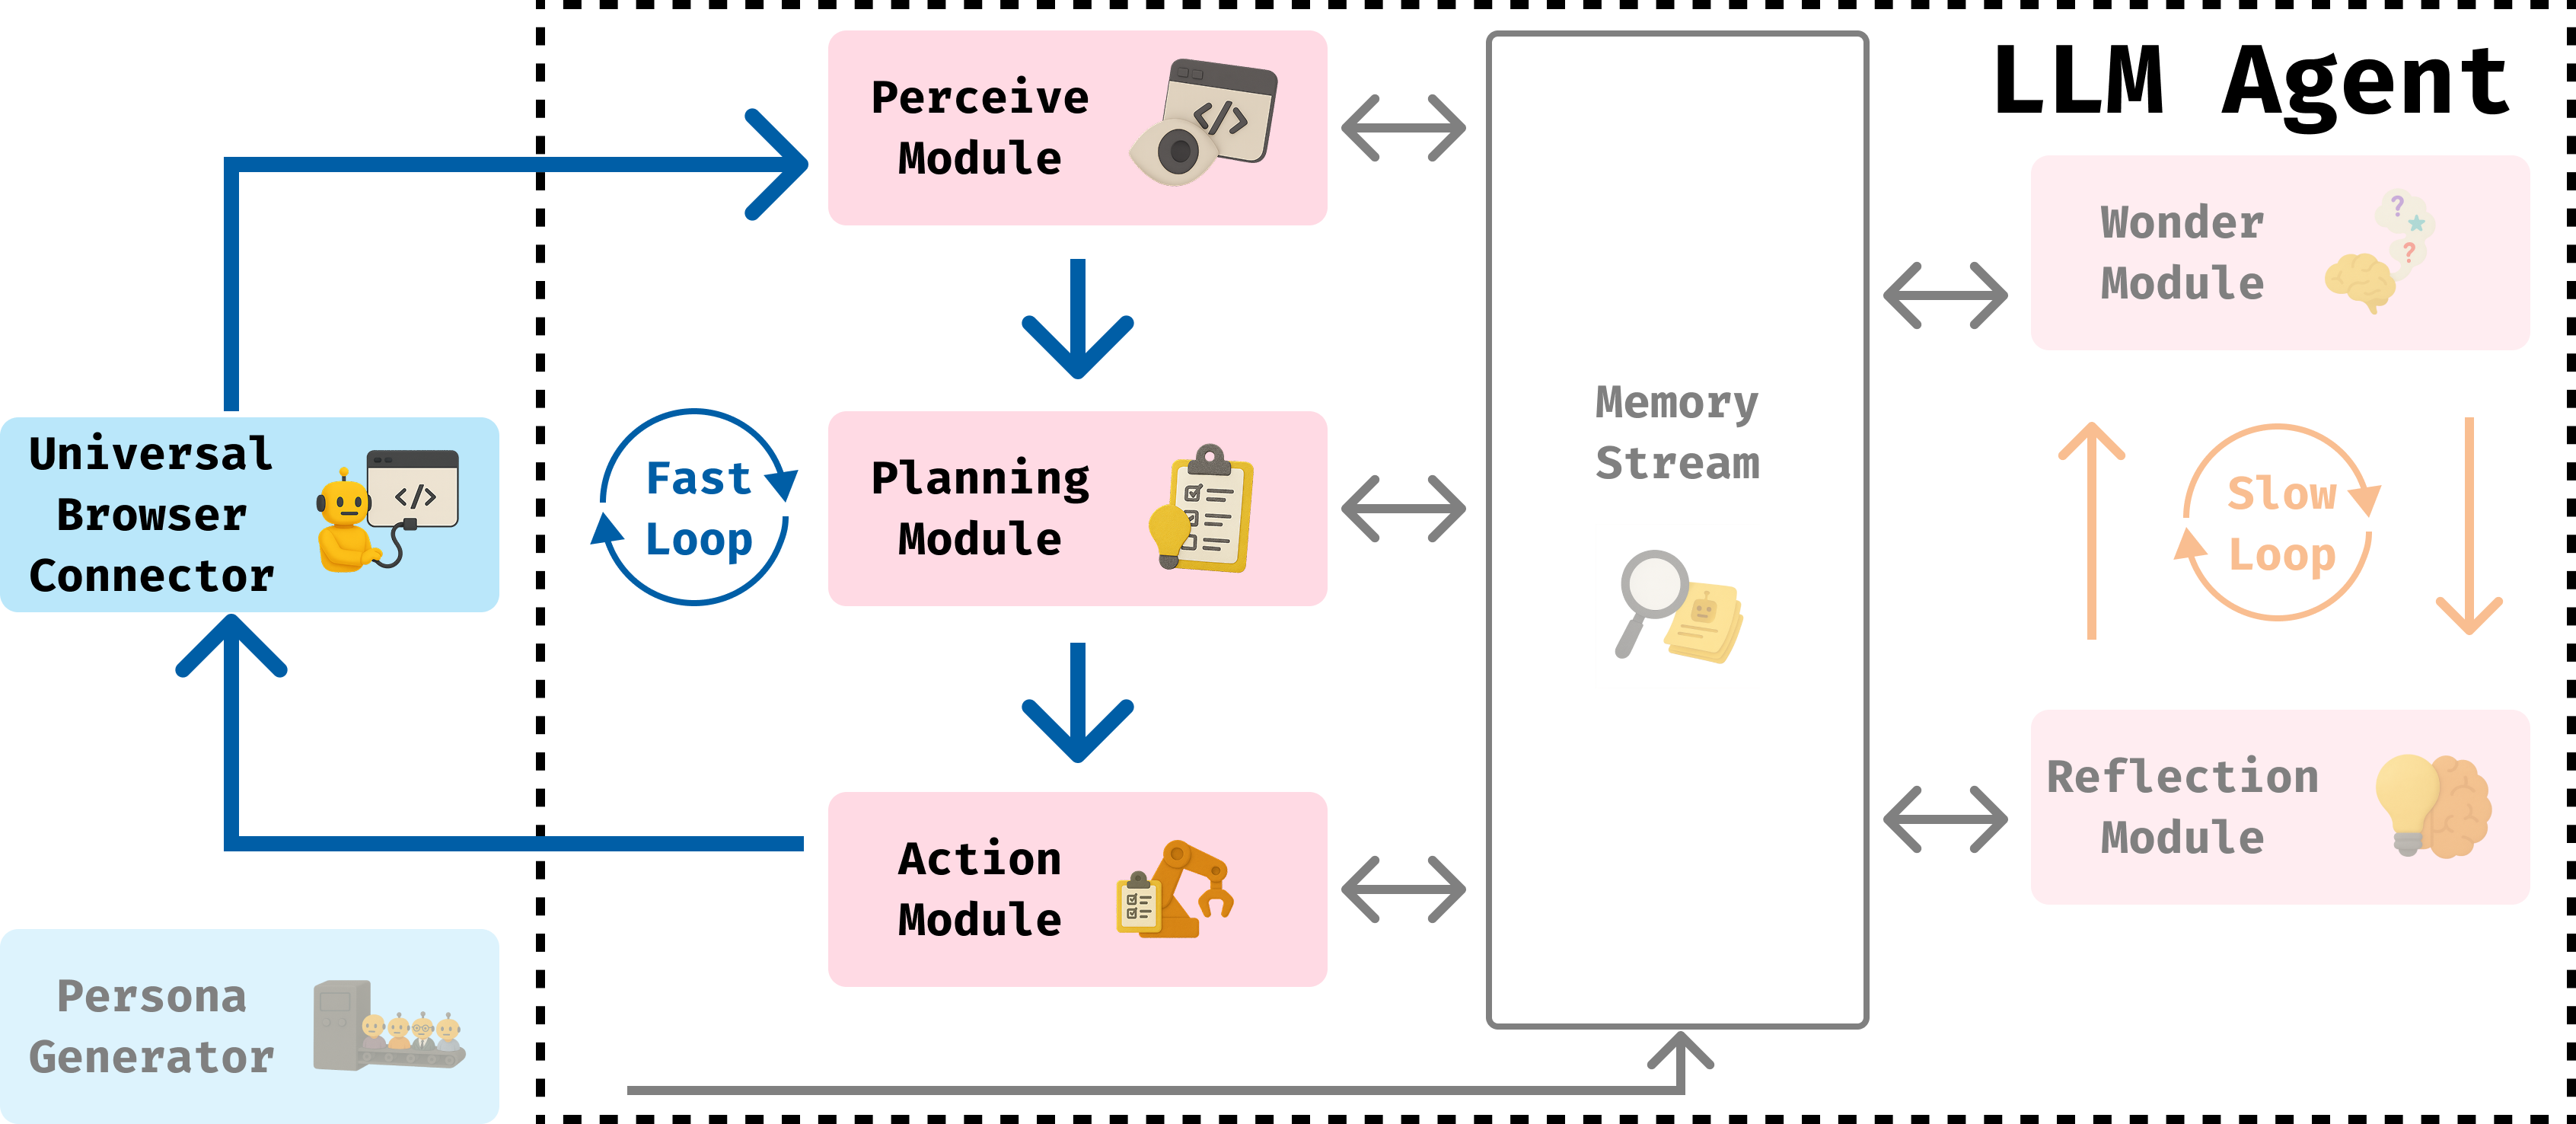
\includegraphics[width=\linewidth]{figures/structure-fast@2x.png}
  \end{figure}
\end{frame}
\begin{frame}{Agent Architecture - Slow Loop}
  \begin{figure}[htp]
    \centering
    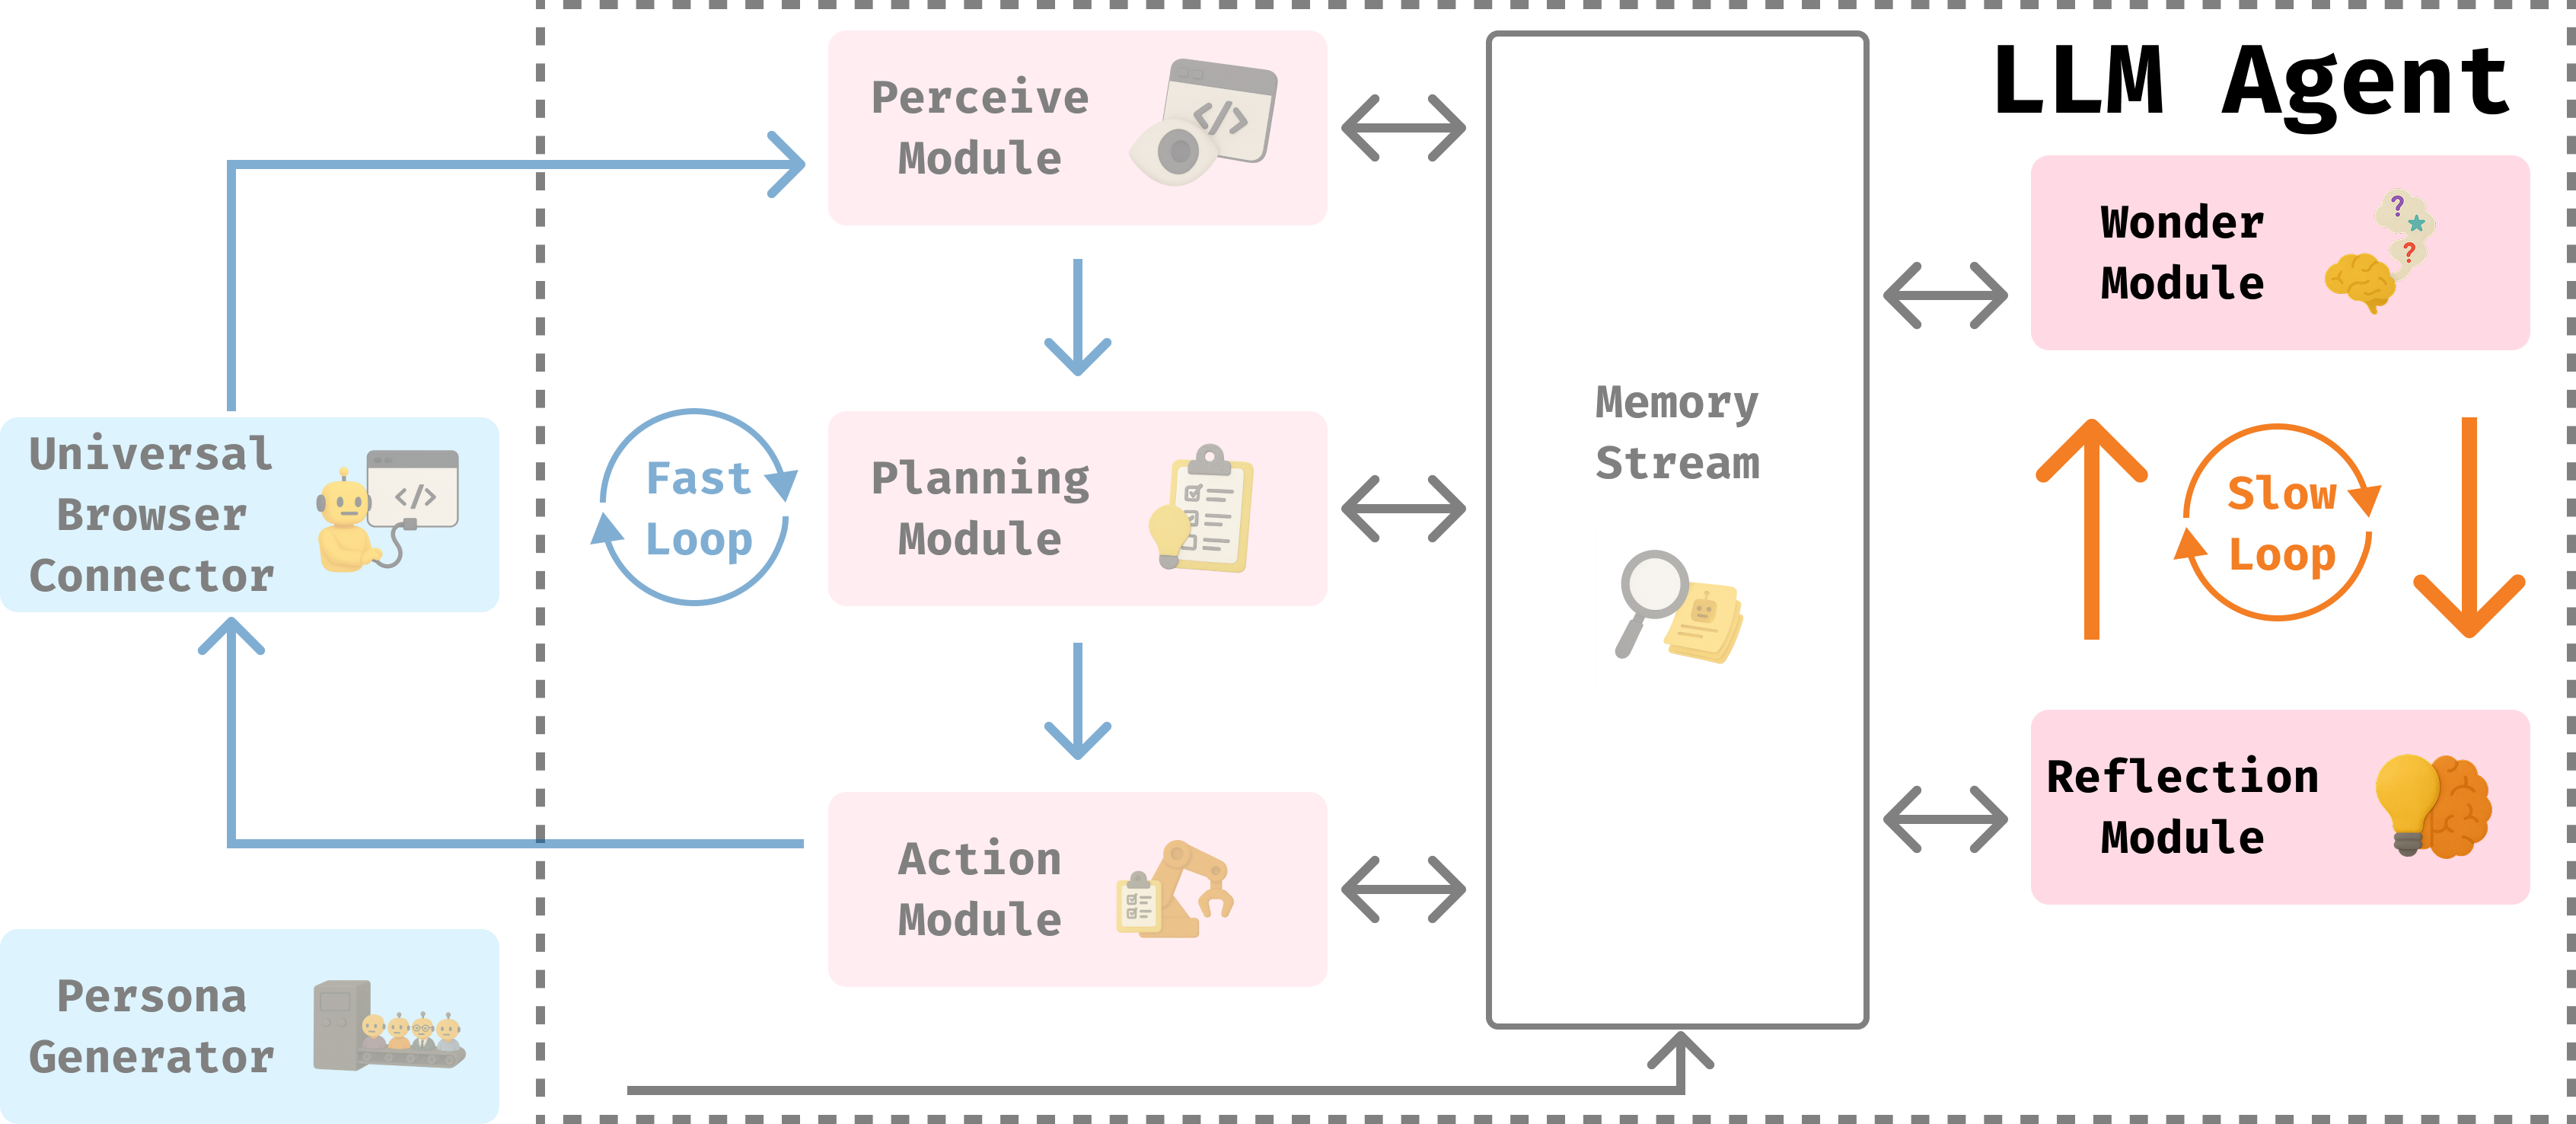
\includegraphics[width=\linewidth]{figures/structure-slow@2x.png}
  \end{figure}
\end{frame}
\begin{frame}{Agent Architecture - Memory Stream}
  \begin{figure}[htp]
    \centering
    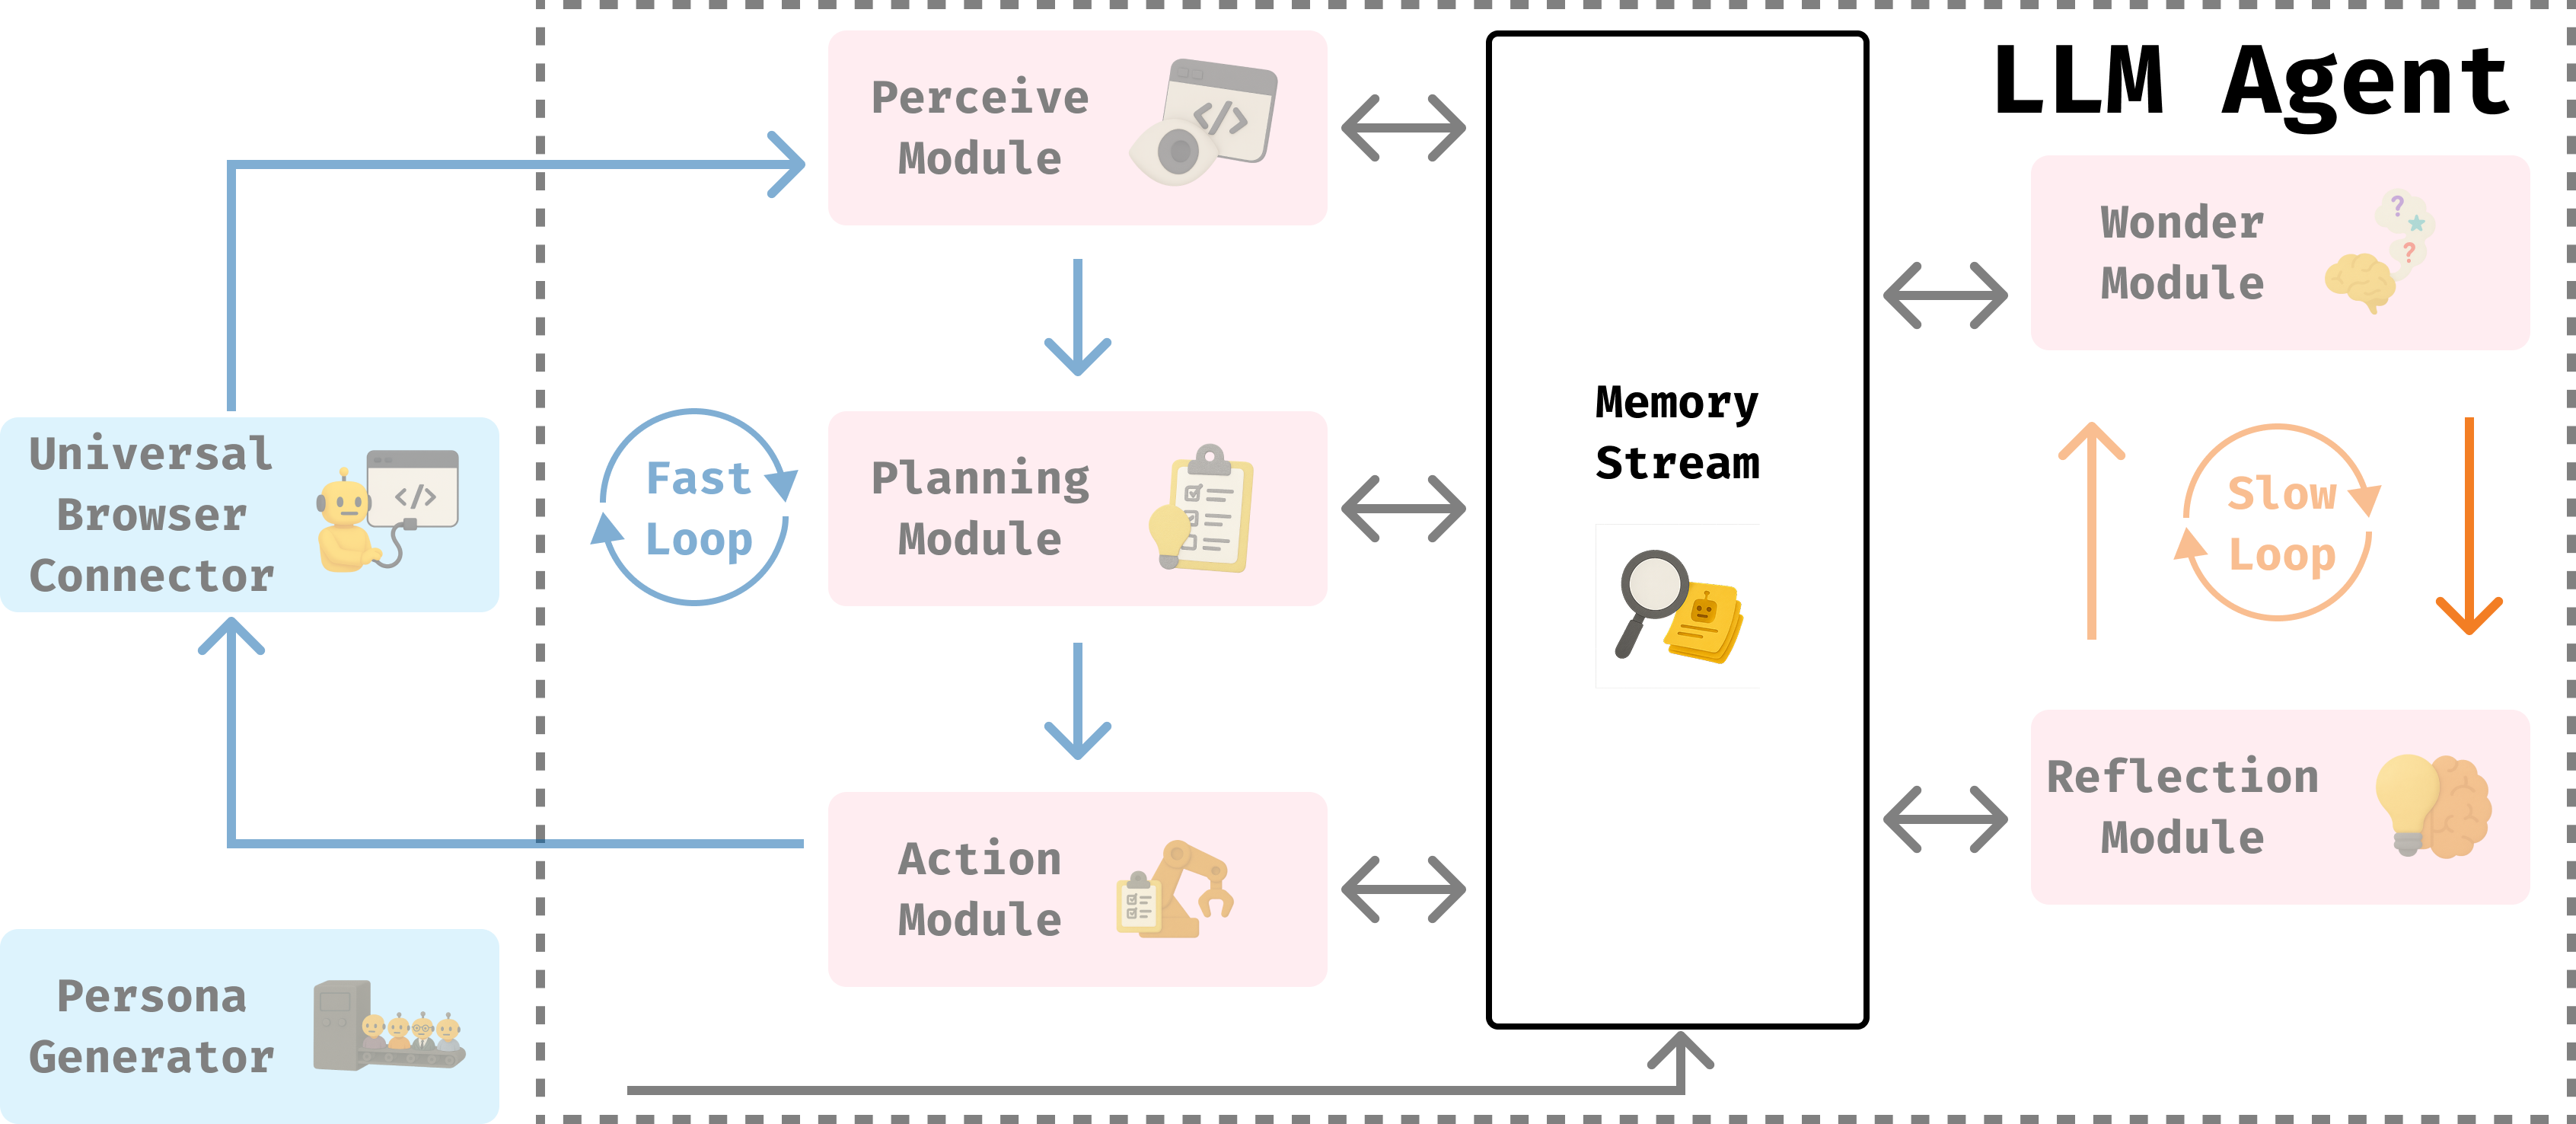
\includegraphics[width=\linewidth]{figures/structure-memory@2x.png}
  \end{figure}
\end{frame}

\begin{frame}{Agent Architecture - Collected Data}
  \begin{figure}[htp]
    \centering
    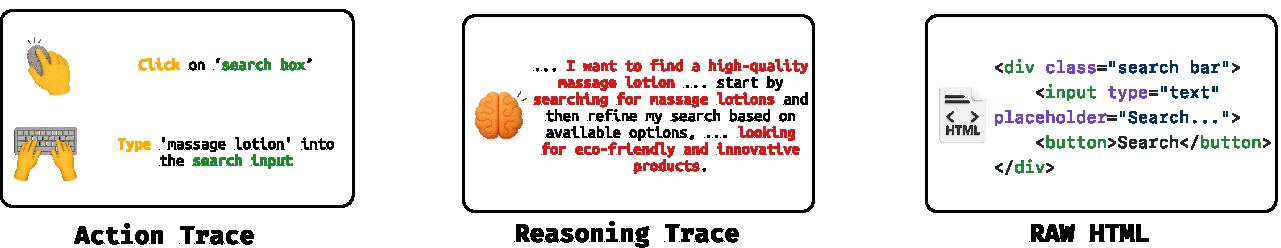
\includegraphics[width=\linewidth]{figures/data_collected.pdf}
  \end{figure}
\end{frame}

% \begin{frame}{Agent Architecture: Two-Loop + Memory}
  
%   \begin{outline}
%     \1 To allow both in-depth reasoning and real-time simulation:
%     \2 Fast Loop: rapid response to the outside environment
%     \2 Slow Loop: in-depth reasoning and thinking
%     \1 Asynchronous; interact through Memory Stream
%     \1 Each module retrieves and generate memories
%     \pause
%     \1 Data collected from our LLM Agent:
%       \2 Action Trace: what the agent did
    
%       \2 Final Session Outcome: final action in the action trace. Completing the task / terminating the session
    
%       \2 Reasoning Trace: agents' internal memory entries for supporting qualitative analysis
%   \end{outline}
% \end{frame}

\begin{frame}{Result Viewer Interface}
  \begin{figure}[htp]
    \centering
    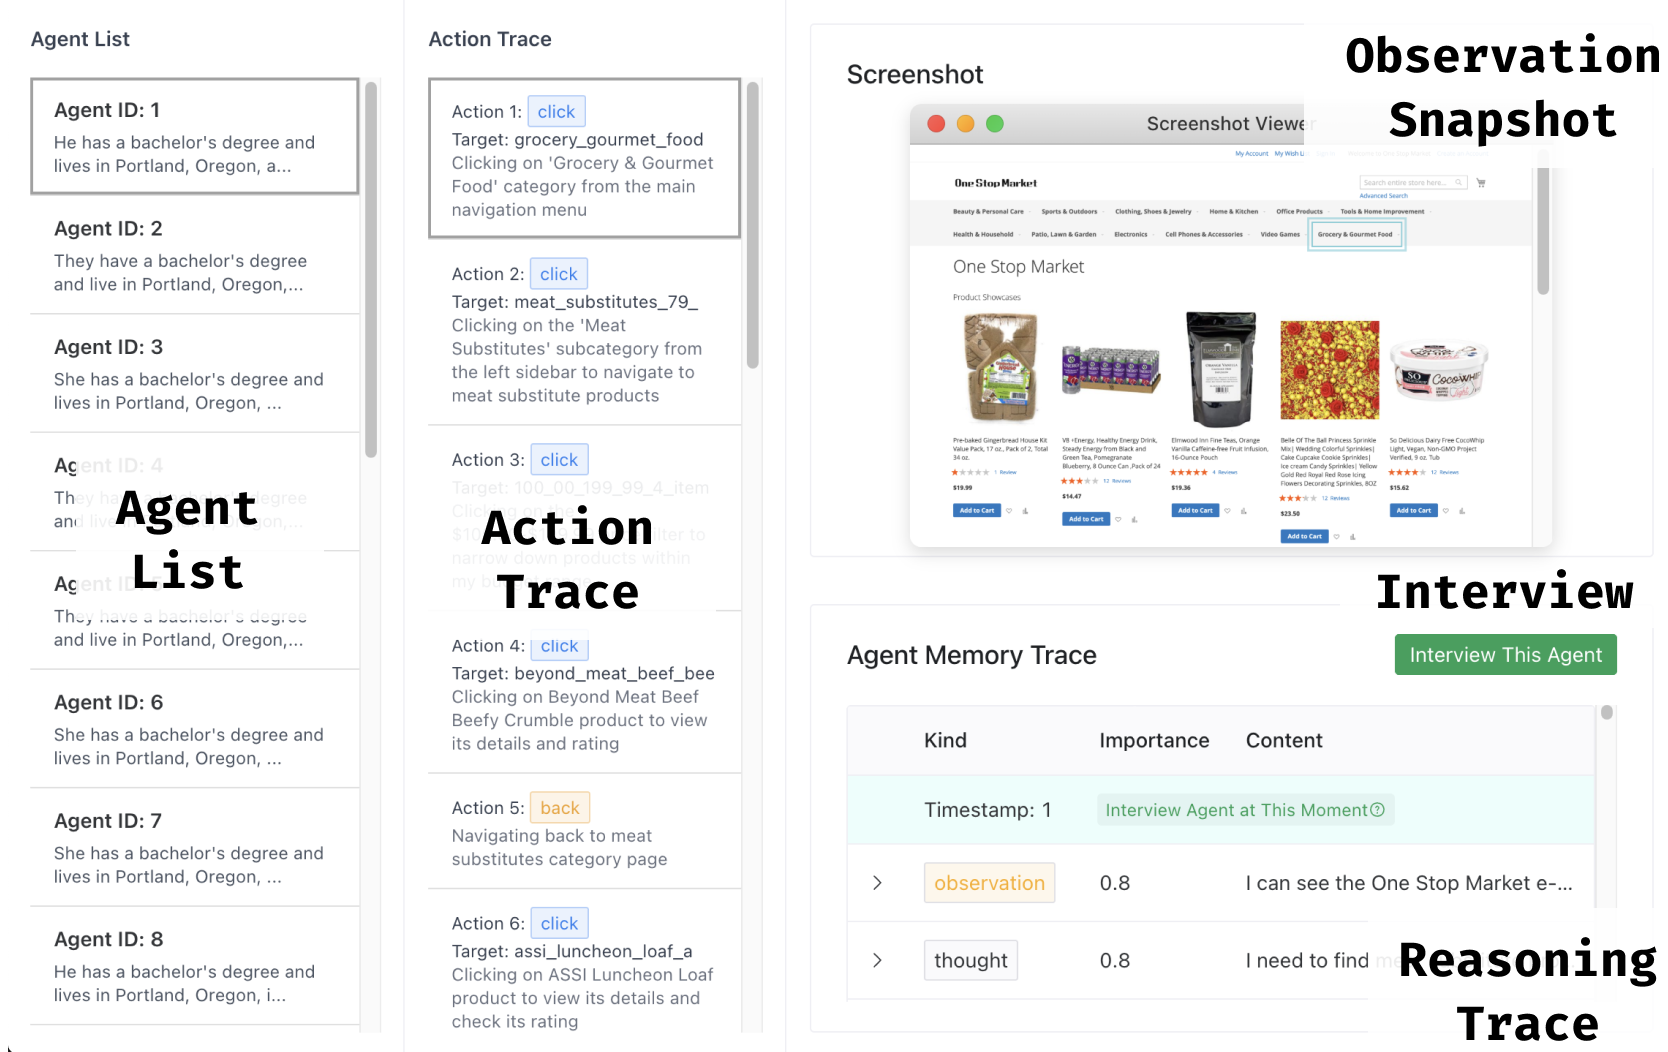
\includegraphics[width=.7\linewidth]{figures/uxagent/result-viewer-detail.png}
    \caption{Result Viewer Interface}
  \end{figure}
\end{frame}

\begin{frame}{Universal Browser Connector}
  \begin{figure}[htp]
    \centering
    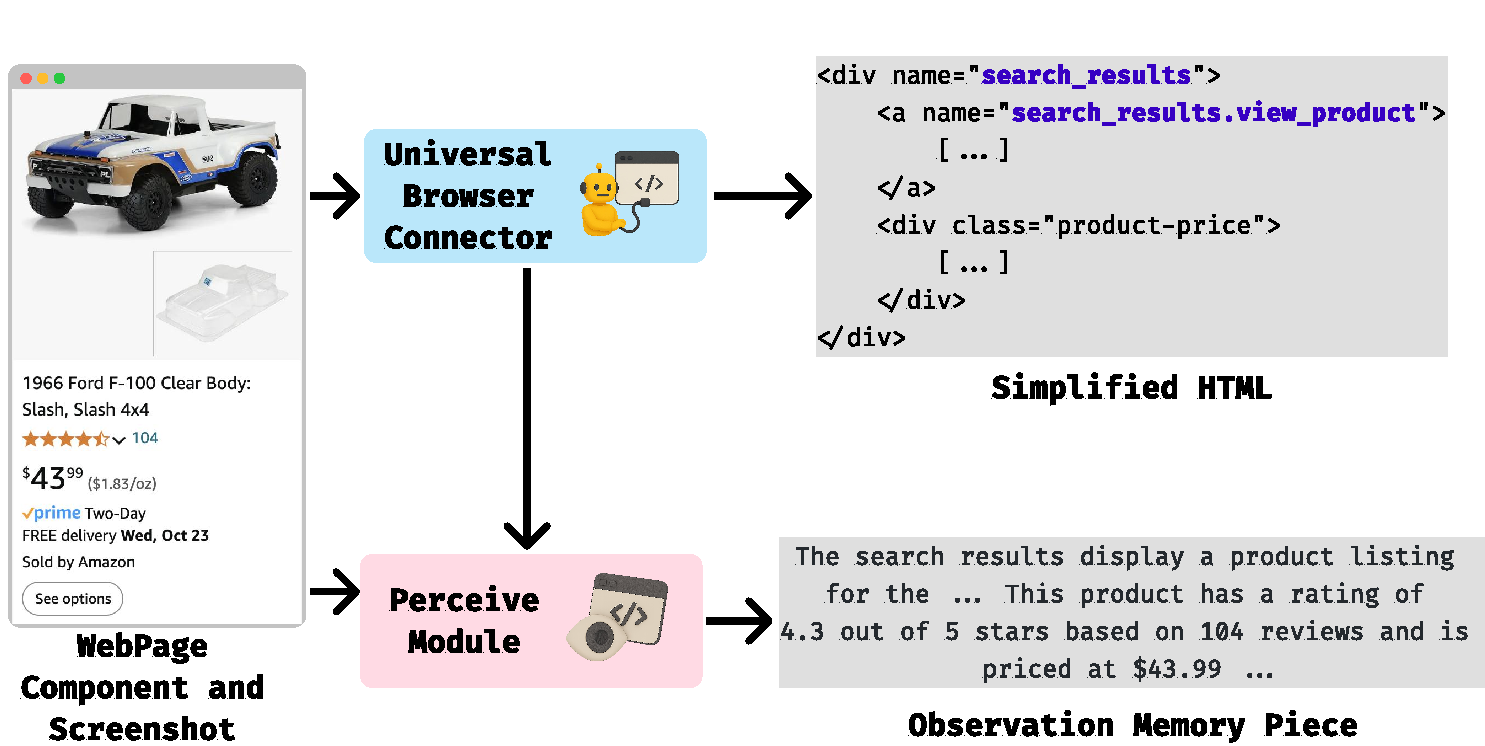
\includegraphics[width=.8\linewidth]{figures/uxagent/perception-demo.pdf}
    \caption{Universal Browser Connector}
  \end{figure}
\end{frame}

\begin{frame}[standout]
  UXAgent Evaluation: can simulated agents help UX researchers?
\end{frame}

\begin{frame}{User Study Setup}
  % check sun lu figure 1
  \begin{outline}
    \1 16 UX researchers
    \1 Reviewed 20 LLM simulated sessions
    \1 Task: buy a meat substitute (highest rating, \$100--200), stop at checkout
    \1 Flow (\textasciitilde 30 min): 
      \2 review draft protocol
      \2 inspect simulated traces/screenshots/reasoning 
      \2 optional agent interview 
      \2 revise protocol and feature ideas 
      \2 survey
  \end{outline}
\end{frame}

\begin{frame}{Post-Study Ratings (Likert -2 to 2)}
  % bar chart

  % quotes
  \begin{outline}
    \1 Usability M=1.63 (SD=0.50); Helpfulness M=1.38 (SD=0.72)
    \1 Trust M=0.63 (SD=0.81); Satisfaction with revised protocol M=1.00 (SD=0.89)
    \1 “LLM can replace humans” M=-0.44 (SD=1.15)
  \end{outline}
\end{frame}

\begin{frame}{Protocol Iteration Outcomes}
  \begin{outline}
    \1 14/16 proposed further study-design changes after using UXAgent
    \1 Edits: tasks (6), demographics (3), survey items (2), interview protocol (2), added metrics (2)
    \1 Typical cadence: build trust $\rightarrow$ sense-making $\rightarrow$ hypothesize/verify (with interviews) $\rightarrow$ converge on revisions
  \end{outline}
\end{frame}

\begin{frame}{Trust and Realism}
  \begin{outline}
    \1 Data seen as useful/rational; some behaviors “not what real users would do”
    % \todo{change to one page with only quote}
    \1 Trust improves with transparency (reasoning trace)
    \1 Position: complement, not replace, human participants—best for early, low-cost iteration
  \end{outline}
  \begin{figure}
    \centering
    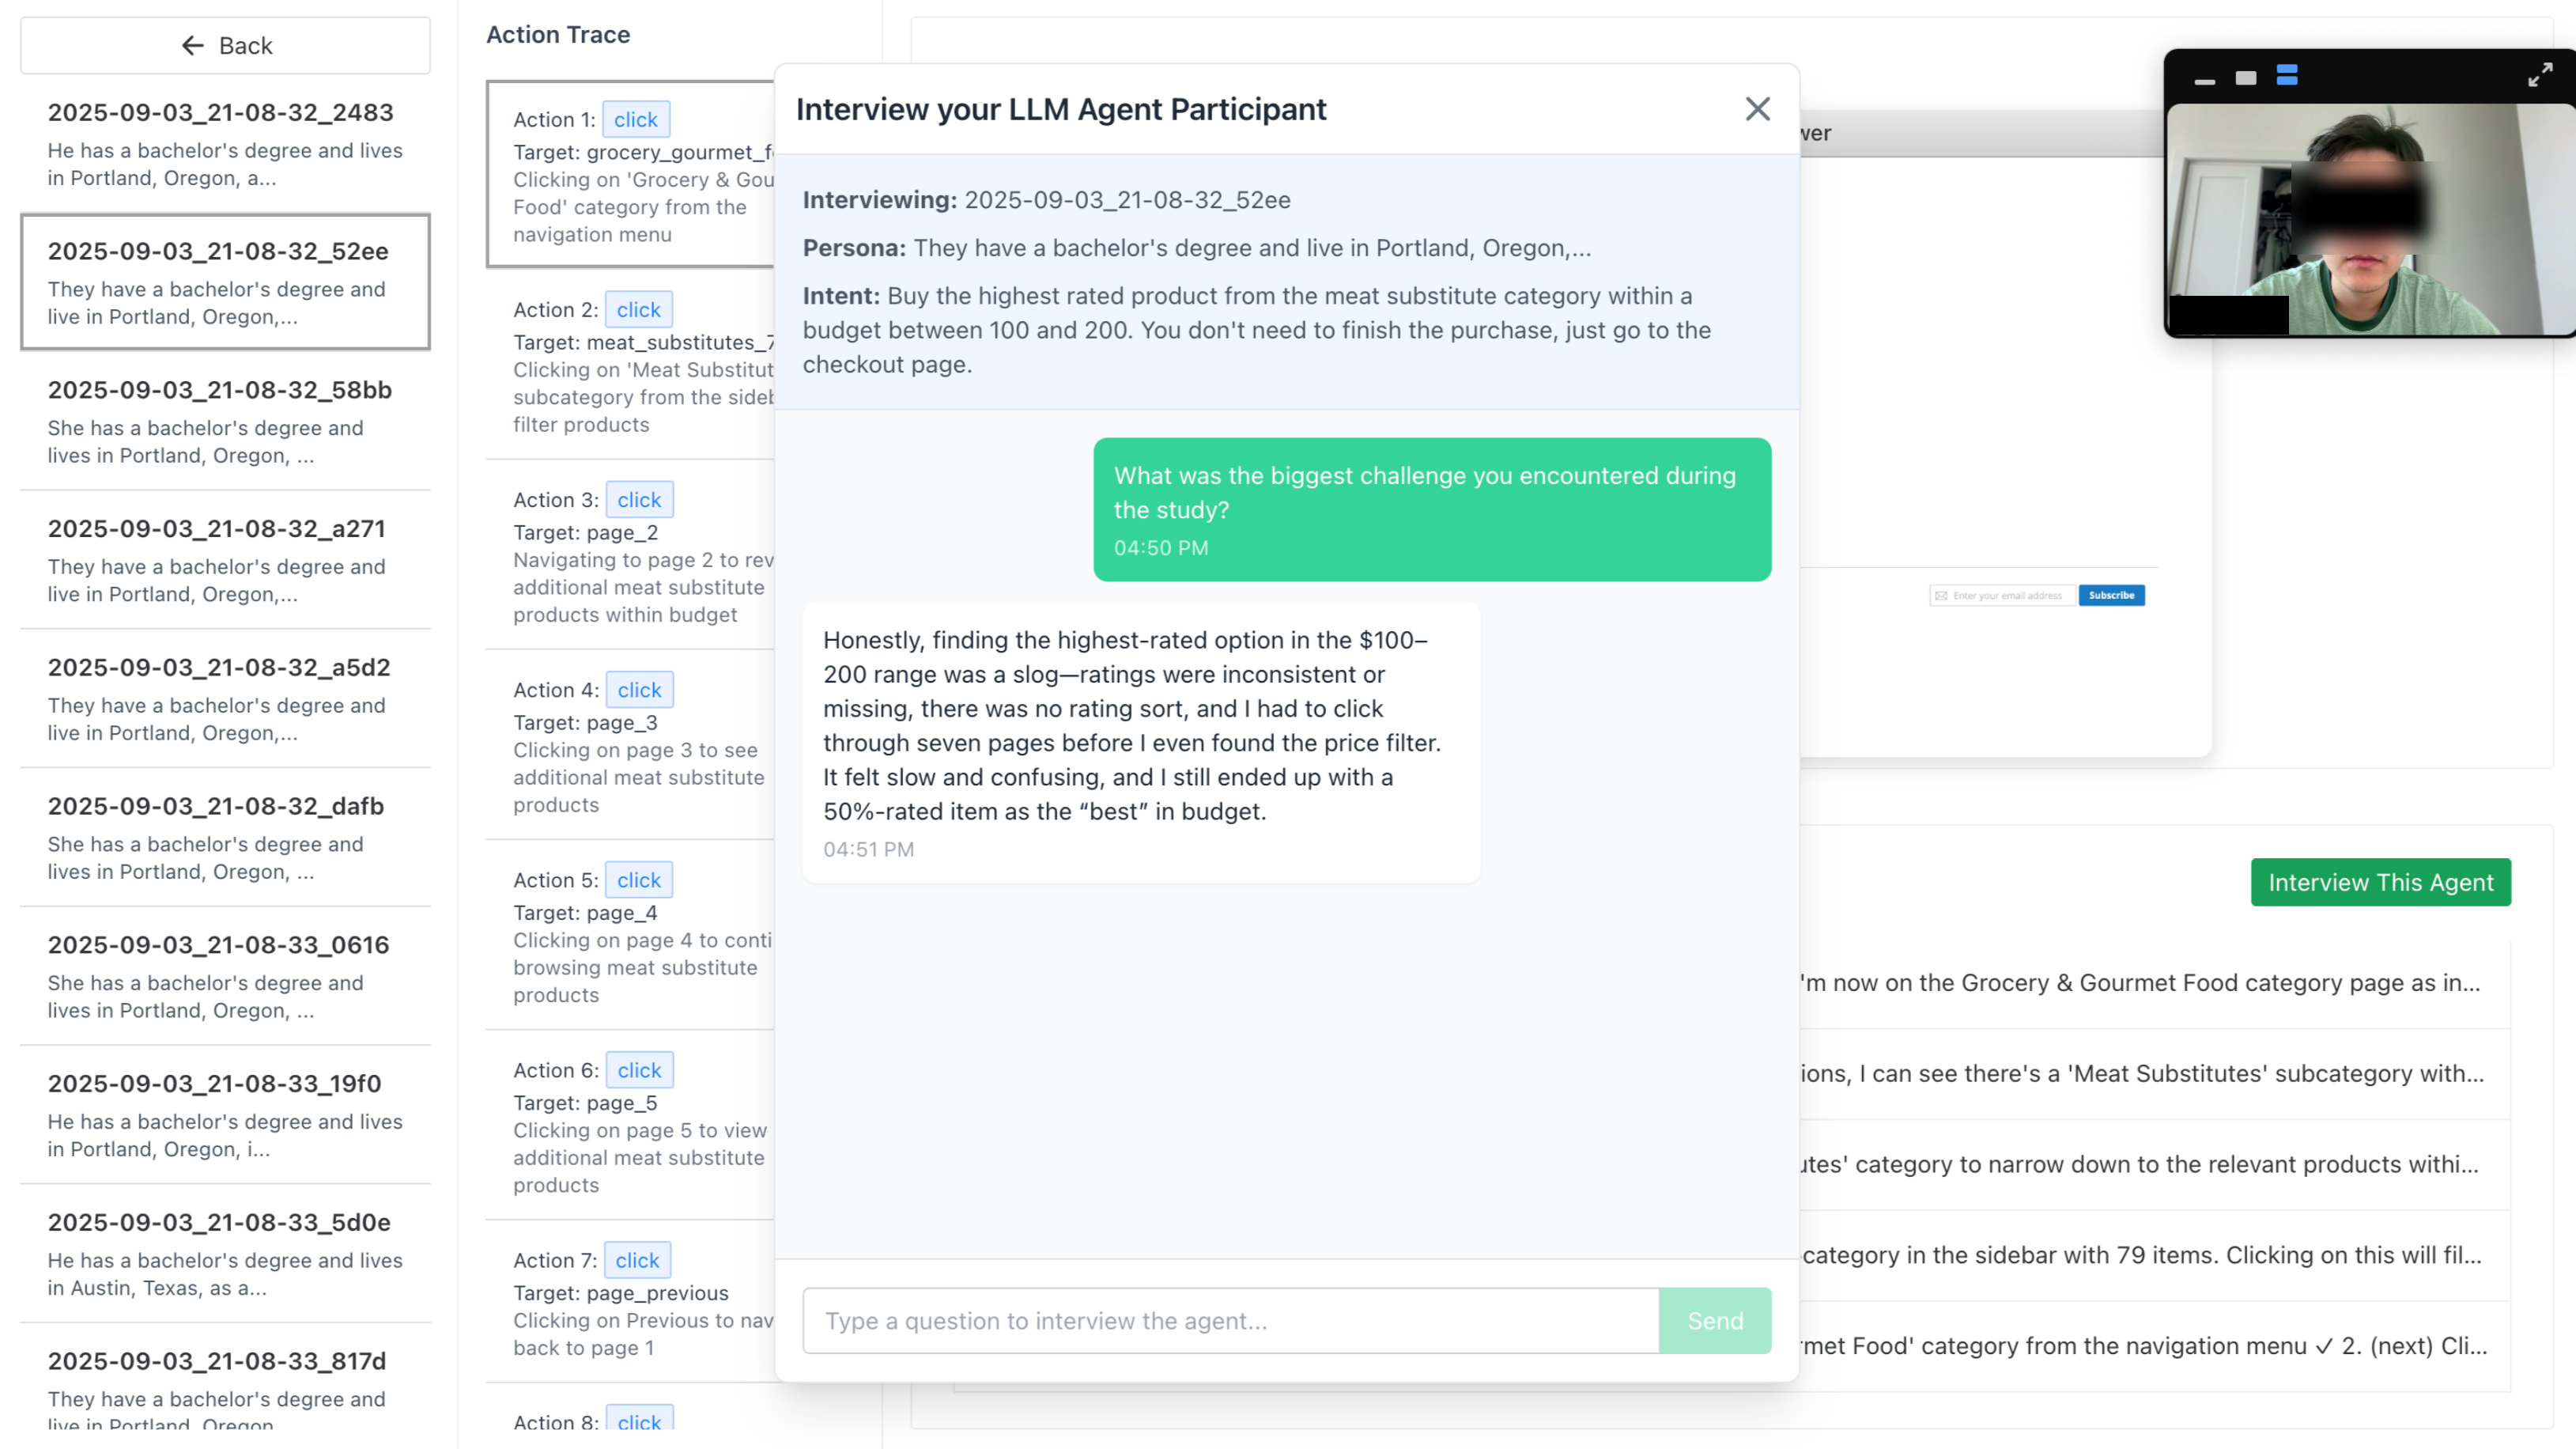
\includegraphics[width=0.5\linewidth]{figures/uxagent/participant.png}
    \caption{Study session with a UX researcher using UXAgent.}
  \end{figure}
\end{frame}

\begin{frame}[standout]
  We've seen UXAgent can help UX researchers ...
  \vspace{10pt}
  \pause

  Remaining question: How accurate are LLM Agents in simulating human behavior?
\end{frame}

\section[Case Study 2: Can LLM Agents Simulate Multi-Turn Human Behavior?]{Case Study 2: Use Real Online Customer Behavior Data to Evaluate and Improve}

% \begin{frame}{Motivation}
%   \begin{outline}
%     \1 Large Language Models (LLMs) have enabled the simulation of ``believable'' human behavior \cite{parkGenerativeAgentsInteractive2023}.
%     \1 Many application areas have emerged:
%       \2 Social Science Studies \cite{parkGenerativeAgentSimulations2024}
%       \2 UX Studies \cite{luUXAgentSystemSimulating2025}
%       \2 A/B Testing Studies \cite{wangAgentAAutomatedScalable2025}
%   \end{outline}
% \end{frame}

% \begin{frame}{Motivation}
%   \begin{outline}
%     \1 However, current systems are primarily optimized for and evaluated by their ``believability'':
%       \2 \textit{``how much people feel it is like a human''}
%     \1 rather than their ``accuracy'':
%       \2 \textit{``how much it acts like a human''}
%     \pause
%     \1 Some work evaluates the final outcomes of tasks (e.g., item purchases) \cite{yaoReActSynergizingReasoning2023}
%     \pause
%     \1 The fidelity of intermediate actions in the sequences are not quantitatively evaluated.
%   \end{outline}
% \end{frame}

% \begin{frame}[standout]
%   How can we better evaluate and improve LLM Agents' action accuracy in simulating human behavior?
% \end{frame}

% \begin{frame}[standout]
%   How can we better evaluate and improve LLM Agents' action accuracy in simulating human \textit{\ul{shopping}} behavior?
% \end{frame}

\subsection*{Task \& Method}

\begin{frame}{Task Definition}
  \begin{outline}
    \1 We focus on the \textbf{human behavior simulation task}
      \2 Generate the next user action based on the context and past actions.
      \2 Specifically, in the online shopping scenario.
  \end{outline}
  \begin{figure}
    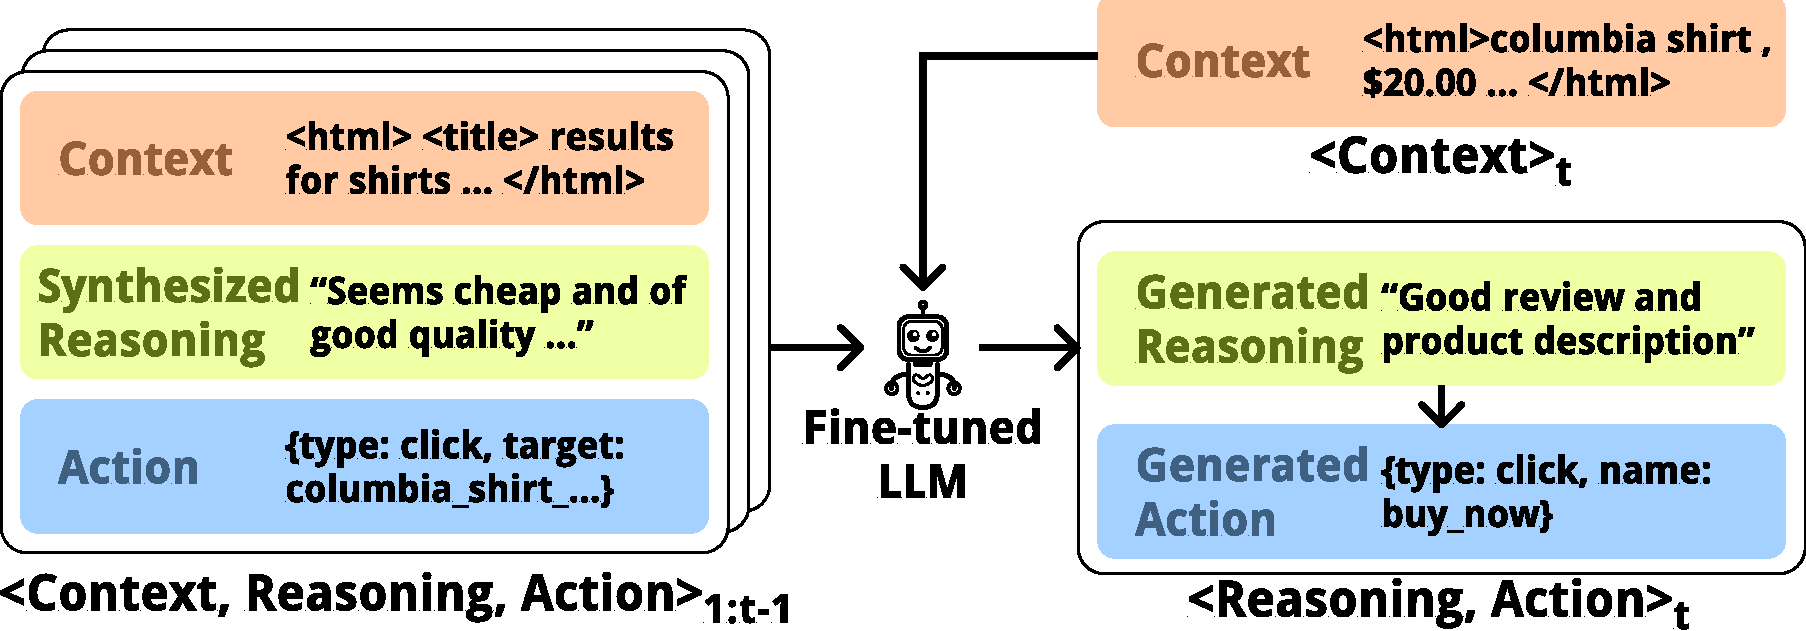
\includegraphics[width=\linewidth]{figures/finetuned_web_agent/teaser.pdf}
    \caption{Overview of the next action prediction task.}
  \end{figure}
\end{frame}

\begin{frame}{Dataset}
  \begin{outline}
    \1 Collected from a real-world online shopping platform.
    \1 31,865 sessions from 3,526 users
    \1 230,965 user actions
    \1 4,432 purchases, 27,433 terminations
  \end{outline}
\end{frame}

\begin{frame}{Context}
  \begin{outline}
    \1 \textbf{Context} (or the ``observation space'') is defined as the a ``simplified'' HTML-based representation of the current page.
    \1 JS and CSS are removed.
    \1 Important structural information (Table, List, etc.) is preserved.
    \1 LLM already understands the HTML format, no need to re-define ``button'' and ``input'' etc.
    \pause
    \1 Each interactable element is assigned a unique ``name'' (e.g. \code{product_form.add_to_cart})
  \end{outline}
\end{frame}
\begin{frame}{Action}
  \begin{outline}
    \1 \textbf{Action} is defined as the next raw browser action conducted by the user.
      \2 Generalizable to other domains beyond online shopping.
    \1 \code{click} (click on an element)
    \1 \code{type_and_submit} (type text and submit a form by hitting enter)
    \1 \code{terminate} (user ends the session by closing the browser window)
  \end{outline}
\end{frame}


\begin{frame}{Reasoning}
  \begin{outline}
    \1 \textbf{Reasoning} is defined as a natural language sentence that describes the reasoning behind an action.
      \2 \textit{``I want to find a comfortable piece of clothing, so I’m looking for options with high ratings.''}
    \1 Enhances the explainability of the model.
    \1 Not present in existing datasets.
  \end{outline}
  
\end{frame}

\begin{frame}{Rationale Synthesis}

  % change to example


  \begin{outline}
    \1 Reasoning traces are crucial for understanding users' action choices
    \1 Difficult to collect; thus, they are often not available in behavioral datasets.
    \1 Reasoning Synthesis Pipeline:
      \2 Record a real human customer's think-aloud shopping sessions as in-context learning examples.
      \2 Provide an LLM with the observation context and the corresponding action.
      \2 Use LLM to generate a free-text reasoning explaining the user's decision.
  \end{outline}  
\end{frame}

\begin{frame}{Finetuning LLMs}
  % loss function, formally define
  \begin{outline}
    \1 To enhance LLMs' accuracy in simulating human behavior, we finetune them on the task.
    \2 \textbf{Input:} ${\langle Context, Reasoning, Action\rangle}_{1:t-1}$ + $<Context>_t$ 
    \2 \textbf{Output:} $\langle Reasoning, Action\rangle _{t}$
    \1 Training:
      \2 Entire session is inputed as a whole.
      \2 Minimize the loss of the predicted action and reasoning tokens
    \1 Inference:
      \2 Input the context, past actions and corresponding reasoning.
      \2 Output the next action and reasoning.
  \end{outline}
\end{frame}

\subsection{Evaluation and Experiments}

\begin{frame}{Evaluation Metrics}
  \begin{outline}
    % \1 Two tasks: 
    \1 Next Action Generation
      \2 Exact Match
      \2 Predicted action is only considered correct if both the action type (click, terminate, etc.) and the action attribute (the click target / the input text) match the ground truth.
      \pause
    \1 Shopping Outcome Prediction
      \2 Essentially predicting the last action based on the session history.
      \2 One of \code{click} on a \code{buy_now} button or \code{terminate} the session.
      \2 F1 score
  \end{outline}
\end{frame}

\begin{frame}{Models}
  \begin{outline}
    \1 Baseline Models:
      \2 Claude
      \2 Llama
      \2 Mistral
      \2 DeepSeek-R1
    \1 Fine-tuned Models:
      \2 Llama
      \2 Qwen
      \2 Mistral
  \end{outline}
\end{frame}

\begin{frame}{Results -- Accuracy \& F1}
  \begin{table}[t]
    \centering
    \footnotesize
    
    \begin{booktabs}{
        width=\linewidth,
        colspec={lcccccc},
        cell{1}{2,5} = {c=3}{},
        cell{1}{1} = {r=2}{},
        column{1}={font=\small},
        row{1,2}={font=\bfseries},
        cell{3,9}{1} = {c=7}{bg=black!30!white,font=\bfseries},
        % row{3,8}={rowsep=4pt},
        cell{11,13,15}{1} = {r},
    }
    \toprule
    Model                & {Next Action Gen.} & & & {Session Outcome} \\
    \cmidrule[r]{2-4} \cmidrule[l]{5-7}
                         & Acc.                & $\%\Delta$ & v.s. DS-R1 & F1 Score             & $\%\Delta$& v.s. DS-R1 \\
    \midrule
    Pre-Trained Models   &                         &                    &                  &                      &                    &                  \\
    DeepSeek-R1          & 11.86\%                 & -                  & -                & 20.01\%              & -                  & -                \\
    Mistral-7B-v0.3      & 4.25\%                  & -                  & \highlightRelevantValue{-7.61} & 11.27\%              & -                  & \highlightRelevantValue{-8.74} \\
    Qwen2.5-7B           & 4.25\%                  & -                  & \highlightRelevantValue{-7.61} & 11.94\%              & -                  & \highlightRelevantValue{-8.07} \\
    Llama 3.2 3B         & 2.93\%                  & -                  & \highlightRelevantValue{-8.93} & 8.60\%               & -                  & \highlightRelevantValue{-11.41} \\
    Claude 3.7 Sonnet    & 9.34\%                  & -                  & \highlightRelevantValue{-2.52} & 12.81\%              & -                  & \highlightRelevantValue{-7.20} \\
    Fine-tuned Models    &                         &                    &                  &                      &                    &                  \\
    Qwen2.5-7B~          & \underline{16.67\%}                 & -                  & \highlightRelevantValue{4.81}  & 26.92\%              & -                  & \highlightRelevantValue{6.91}  \\
    + reasoning          & \textbf{17.26\%}                 & \highlightRelevantValue{3.54}  & \highlightRelevantValue{5.40}  & \underline{ 33.86\%}              & \highlightRelevantValue{25.78} & \highlightRelevantValue{13.85} \\
    Mistral-7B-v0.3~     & 14.17\%                 & -                  & \highlightRelevantValue{2.31}  & 17.99\%              & -                  & \highlightRelevantValue{-2.02} \\
    + reasoning          & 15.84\%                 & \highlightRelevantValue{11.79}  & \highlightRelevantValue{3.98}  & 30.12\%              & \highlightRelevantValue{67.43}  & \highlightRelevantValue{10.11} \\
    Llama-3.2-3B~        & 9.31\%                  & -                  & \highlightRelevantValue{-2.55} & 4.73\%               & -                  & \highlightRelevantValue{-15.28} \\
    + reasoning          & 15.77\%                 & \highlightRelevantValue{69.39}  & \highlightRelevantValue{3.91}  & \textbf{33.99\%}              & \highlightRelevantValue{618.60} & \highlightRelevantValue{13.98} \\
    \bottomrule
    \end{booktabs}
    \caption{Model performance.}
    % \vspace{2\baselineskip}
    \label{tab:results}
    \end{table}
\end{frame}

\begin{frame}{Results -- Distribution}
  \begin{figure}
    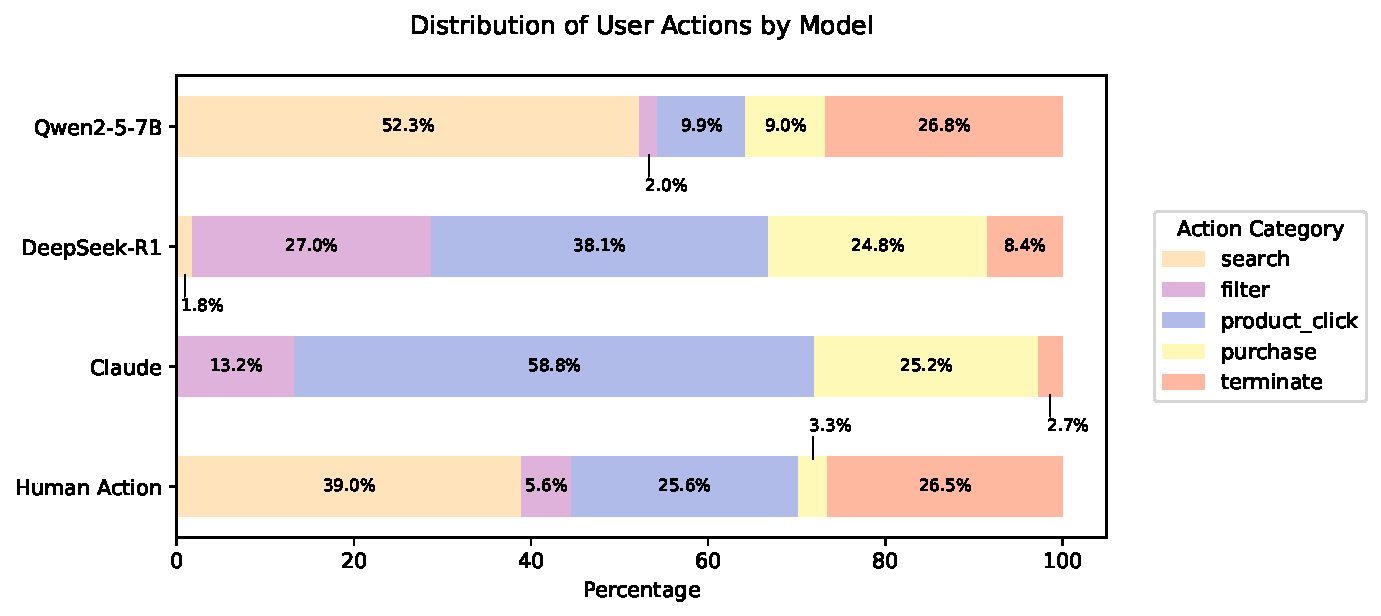
\includegraphics[width=\linewidth]{figures/finetuned_web_agent/action_distribution_below_labels.pdf}
    \caption{Distribution of the action types in the dataset.}
  \end{figure}
\end{frame}

% \begin{frame}{Ablation Study}
%   \begin{outline}
%     \1 To evaluate the impact of training model with synthesized reasoning trace, we conduct an ablation study \textbf{to remove the reasoning trace} from the training data.

%   \end{outline}
%   \begin{table}[t]
%     \centering
%     \begin{booktabs}{
%       colspec = {X[l]cc},
%       cells={m},
%       cell{3,5,7}{1}={r,font=\itshape},
%     }
%     \toprule
%     Model                         & { Action Gen. \\\ (Acc.) }& {Outcome \\ (F1)} \\
%     \midrule 
%     Qwen2.5-7B SFT                    & \textbf{17.26\% }            & 33.86\%            \\
%     w/o reasoning                 & 16.67\%             & 26.92\%            \\
%     Mistral-7Bv0.3 SFT               & 15.84\%             & 30.12\%            \\
%     w/o reasoning                 & 14.17\%             & 17.99\%            \\
%     Llama-3.2-3B SFT                  & 15.77\%             & \textbf{33.99\%}            \\
%     w/o reasoning                 & 9.31\%              & 4.73\%             \\
%     \bottomrule
%     \end{booktabs}
%     \caption{Ablation study result.}
%     \label{tab:ablation}
%     \end{table}
% \end{frame}

% \begin{frame}{Error Analysis}
%   \begin{outline}
%     \1 We analyze the errors made by the models: Claude and Qwen 2.5 7B.
%     \1 Error types\footnote{Illegal actions generated by models are excluded from this analysis.}:
%       \2 Didn't terminate
%       \2 Didn't click
%       \2 Didn't search
%       \2 Searched wrong keyword
%       \2 Clicked wrong button
%   \end{outline}
% \end{frame}

% \begin{frame}{Error Analysis}
%   \begin{figure}
%     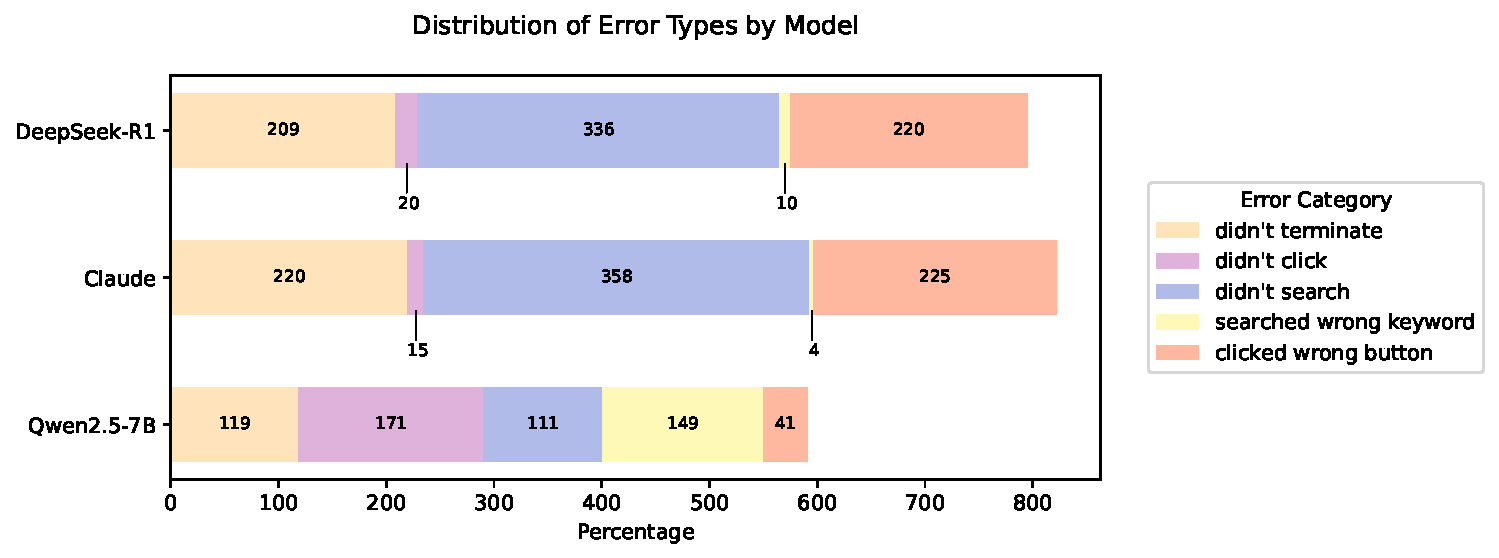
\includegraphics[width=\linewidth]{figures/finetuned_web_agent/error_analysis.pdf}
%     \caption{Error analysis.}
%   \end{figure}
% \end{frame}

% \section{Conclusion}

% \begin{frame}{Conclusion}
%   \begin{outline}
%     \1 We present the first quantative, process-centric evaluation of LLMs for simulating human behavior in online shopping.
%     \1 State-of-the-art models cannot simulate human behavior accurately, i.e. \textit{Prompting is not all-you-need!}
%     \1 Fine-tuning with reasoning traces significantly improves the accuracy of LLMs in simulating human behavior.
%   \end{outline}
% \end{frame}

\begin{frame}[c]
  Supervised fine-tuning improves simulation accuracy, but it remains fundamentally limited.

  As an off-policy learning paradigm, SFT can only reproduce behaviors present in offline data or teacher-generated traces, rather than explore and learn new strategies.

  This places an inherent ceiling on performance.

  Beyond supervised fine-tuning, how can reinforcement learning further improve LLMs for human behavior simulation?
\end{frame}

\section[WebServ: Browser-Server Environment for RL Web Agents]{WebServ: A Browser-Server Environment for Efficient Training of Reinforcement Learning-based Web Agents at Scale}


\begin{frame}{Web Browsers are NOT RL-Ready}
  \begin{outline}
    \1 Web Browsers are NOT RL-Ready:
      \2 Requires per-site configuration or rely on site features
      \2 Noisy context and action
  \end{outline}
\end{frame}

\begin{frame}{Web Servers are NOT RL-Ready}
  \begin{outline}
    \1 Web Servers are NOT RL-Ready
      \2 Expensive, slow, large image size
      \2 Single agent per server (lack of isolation)
      \2 Rollout is expensive
  \end{outline}
\end{frame}

\begin{frame}{System Architecture}
  % \begin{columns}[c]
  %   \begin{column}{0.48\linewidth}
  %     \textbf{Isolation vs. scalability.} Existing web environments rely on a shared server container that leads to cross-agent interference; \projectname creates lightweight per-agent containers to ensure isolation and scalable rollouts for RL training.
  %   \end{column}
  %   \begin{column}{0.52\linewidth}
      \begin{figure}
        
\includegraphics[width=.45\linewidth]{figures/webserv/teaser.png}
        % \caption{System architecture of \projectname.}
      \end{figure}
  %   \end{column}
  % \end{columns}
\end{frame}

% \begin{frame}{Observation Space}
%   \begin{outline}
%     \1 Observation Space: Compact, site-agnostic, generated from webpage DOM.
%       \2 Remove invisible or irrelevant nodes.
%       \2 Preserve interactivity cues (cursor styles).
%       \2 Provide stable, semantically meaningful IDs.
%   \end{outline}
% \end{frame}

% \begin{frame}{Action Space}
%   \begin{outline}
%     \1 Action Space: Minimal, human-aligned operations.
%       \2 Click, type\_and\_submit, select, etc.
%       \2 Simple parameters pointing to IDs.
%   \end{outline}
% \end{frame}

% \begin{frame}{Action Execution}
%   \begin{outline}
%     \1 Robust action executor for SPAs.
%       \2 Network-aware waiting until page settles.
%       \2 Generalizes across sites.
%   \end{outline}
% \end{frame}

% \begin{frame}{Server Stack}
%   \begin{outline}
%     \1 Incus-based manager with block-level COW.
%       \2 Fast launch, clone, reset.
%       \2 Works with existing Docker images.
%       \2 Supports 200+ concurrent containers on one host.
%   \end{outline}
% \end{frame}

\begin{frame}{Evaluation Highlights}
  \begin{outline}
    \1 \projectname + Claude 4.5: 40.0\% (Shopping), 62.9\% (CMS), 50.0\% (GitLab) on WebArena-Lite.
    \1 Faster spin-up: launch latency \textbf{$\sim$5$\times$} faster.
    \1 Storage: \textbf{$\sim$240$\times$} smaller persistent storage.
    \1 200+ concurrent containers on a single host.
  \end{outline}
\end{frame}

\begin{frame}{Benchmarks vs. Vanilla WebArena}
  \begin{table}[t]
    \centering
    \begin{booktabs}{
      colspec = {l l c c c},
      row{1} = {font=\bfseries}
    }
    \toprule
    Environment & Model & Shopping & CMS & GitLab \\
    \midrule
    Vanilla WebArena & GPT-4o       & 11.1 & 20.0 & 10.0 \\
    Vanilla WebArena & OpenAI-o3    & 33.3 & 45.7 & 46.7 \\
    Vanilla WebArena & Llama-3.1-8B & 8.9  & 5.7  & 10.0 \\
    \midrule
    \projectname & GPT-4o       & 20.0 & 28.6 & 43.3 \\
    \projectname & OpenAI-o3    & 37.8 & 48.6 & 46.7 \\
    \projectname & Llama-3.1-8B & 11.1 & 11.4 & 16.7 \\
    \bottomrule
    \end{booktabs}
    \caption{Single-prompt success rate (\%) on WebArena-Lite. \projectname lifts accuracy across proprietary and open-source models.}
  \end{table}
\end{frame}

% \begin{frame}{Ablation: Visual Cues}
%   \begin{table}[t]
%     \centering
%     \scriptsize
%     \begin{booktabs}{
%       colspec={lccc},
%       row{1}={font=\bfseries}
%     }
%     \toprule
%     Model & $\Delta$ Shopping & $\Delta$ CMS & $\Delta$ GitLab \\
%     \midrule
%     GPT-4o & \highlightRelevantValue{-33.3} & \highlightRelevantValue{-70.0} & \highlightRelevantValue{-46.2} \\
%     GPT-5 & \highlightRelevantValue{-18.8} & \highlightRelevantValue{-35.0} & \highlightRelevantValue{-25.0} \\
%     Claude 3.5 Sonnet & \highlightRelevantValue{-58.3} & \highlightRelevantValue{-45.5} & \highlightRelevantValue{-81.8} \\
%     Claude 3.7 Sonnet & \highlightRelevantValue{-50.0} & \highlightRelevantValue{-53.8} & \highlightRelevantValue{-66.7} \\
%     Claude 4 Sonnet & \highlightRelevantValue{-26.3} & \highlightRelevantValue{-29.4} & \highlightRelevantValue{-33.3} \\
%     Claude 4.5 Sonnet & \highlightRelevantValue{-5.6} & \highlightRelevantValue{-45.5} & \highlightRelevantValue{6.7} \\
%     \bottomrule
%     \end{booktabs}
%     \caption{Removing cursor/interaction visual cues hurts most models; weaker models drop more.}
%   \end{table}
% \end{frame}

% \begin{frame}{Ablation: Vision Signals}
%   \begin{table}[t]
%     \centering
%     \scriptsize
%     \begin{booktabs}{
%       colspec={lccc},
%       row{1}={font=\bfseries},
%       cell{3,5}{1}={r}
%     }
%     \toprule
%     Model & Shopping & CMS & GitLab \\
%     \midrule
%     Claude 4 Sonnet (text) & 42.2 & 48.6 & 50.0 \\
%     + VLM & 44.4 & 48.6 & 43.3 \\
%     Claude 4.5 Sonnet (text) & 40.0 & 62.9 & 50.0 \\
%     + VLM & 37.8 & 65.7 & 56.7 \\
%     \bottomrule
%     \end{booktabs}
%     \caption{Vision helps selectively; not universally beneficial across tasks.}
%   \end{table}
% \end{frame}

\begin{frame}{System Efficiency}
  \begin{table}[t]
    \centering
    \begin{booktabs}{
      colspec = {l c c},
      row{1} = {font=\bfseries}
    }
    \toprule
    Metric & \projectname (Incus) & Naïve Docker \\
    \midrule
    Launch speed & 1.781\,s & 8.963\,s \\
    Storage & 28.01\,MiB & 6.78\,GiB \\
    Memory & 1.74\,GiB & 1.63\,GiB \\
    \bottomrule
    \end{booktabs}
    \caption{Incus-based containers cut launch latency ($\sim$5$\times$) and storage ($\sim$240$\times$) at similar RAM.}
  \end{table}
\end{frame}


\begin{frame}{Recap}
  \begin{outline}
    \1 Designing: UXAgent shows how LLM agents can support UX researchers before running costly human studies.
    \1 Evaluating: real behavioral data shows that current agents are still far from faithfully simulating humans.
    \1 Improving: WebServ provides the infrastructure needed to train and improve web agents with reinforcement learning.
  \end{outline}
\end{frame}

\begin{frame}[plain]
  \begin{figure}[htp]
    \centering
    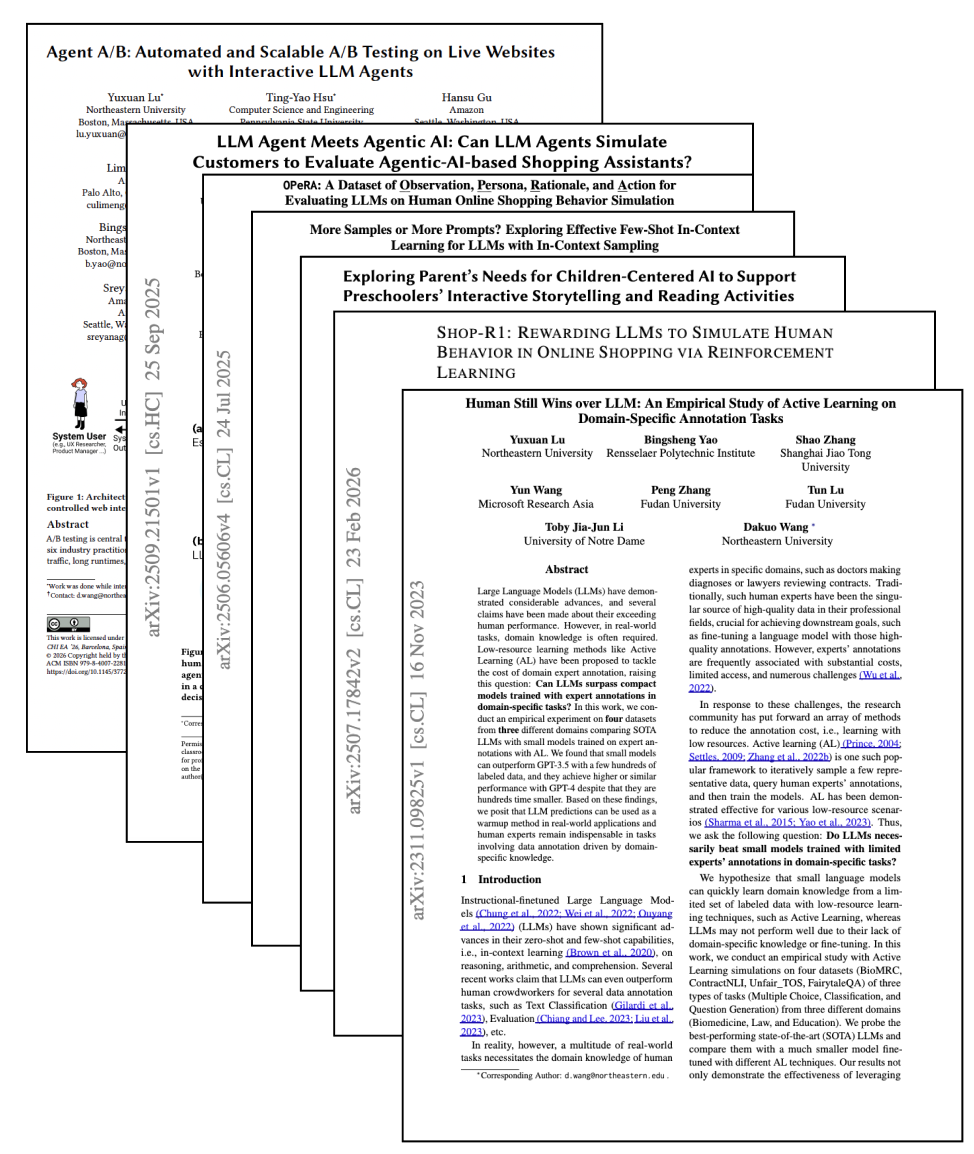
\includegraphics[height=\textheight]{papers.png}
    % \caption{}
  \end{figure}
\end{frame}

\begin{frame}[standout]
  \Large Thank you!

  Questions?

  \begin{tikzpicture}[remember picture,overlay]
    \node[anchor=south east] at ([xshift=-0.8cm,yshift=0.8cm]current page.south east) {
      \qrcode[height=2cm]{https://yuxuan.lu}
    };
  \end{tikzpicture}
\end{frame}

\end{document}
